\typeout{NT FILE STATE-ART.tex}%
\chapter{Background and Related Work}%
\label{ch:state-art}
%
\begin{quote}
\begin{flushright}
``\emph{We stand on the shoulders of giants.}'' \\
\textbf{-- Isaac Newton}, mathematician, physicist, astronomer
\end{flushright}
\end{quote}

In this chapter some background is provided concerning mixed criticality
systems, its relevance and the challenges it poses, alongside with the current
approach to address its complexity. Next, \glsxtrfull{uav} are discussed,
namely the reference hardware and software, both as open-source and commercial
solutions. Lastly, the related work is
presented, showing the current research directions and topics.

% \section{Mixed criticality systems}%
% \label{sec:mixed-crit-syst}
% Embedded systems have stringent requirements both on timing and criticality of
% the tasks it performs. The former concerns the task's timing deadlines
% requirement (firm, soft, hard), whereas the latter is a
% designation of the level of assurance against failure needed for a system
% component~\cite{burns2022mixed}. Typical names for the criticality levels are
% \glspl{asil}, \glspl{dal}, and \glspl{sil}~\cite{burns2022mixed}.

% This is the case for \gls{uav}'s applications with real-time constraints but
% with mixed
% criticality levels, i.e., the risk of failure is more severe in some case than others.
% For example, flight control (safety-critical) and video streaming (non-critical)
% coexist. A compromise in video software could cascade to flight systems, causing
% catastrophic failure—yet strict hardware separation increases weight and reduces
% flight time.

% This exemplifies a \gls{mcs}, i.e., a system comprised of computer hardware and
% software that executes several tasks/applications of distinct criticality (safety) levels.
% However, the integration of mixed-criticality components onto a common hardware
% platform is not an easy task: the designer needs to meet the stringent
% \gls{swap-c} metrics and safety requirements
% provided by safety-critical standards, such as those for automotive~\cite{iso26262}, avionics~\cite{rtca1992software},
% and railway~\cite{cenelec201250128} industries.
% While \gls{mcs} challenges are well-studied in automotive/avionics, UAVs face unique
% constraints: extreme SWaP-C limitations and the need for fail-operational safety
% in uncontrolled environments. Current solutions either compromise isolation
% (single-board) or add weight/energy overhead (multi-board).

% As a result of this integration
% complexity increases, requiring higher computational power, and thus, these
% hardware platforms are migrating from single cores to multi-cores and in the
% future many-core architectures~\cite{burns2022mixed}. This leads to the
% fundamental question of how to reconcile the
% conflicting requirements of \emph{partitioning} for (safety) assurance and \emph{sharing} for
% efficient resource usage. Consequently, problems arise in the modelling, design,
% implementation, and verification of the required \gls{hw} and
% \gls{sw}~\cite{burns2022mixed}.

% Two major areas of research stem from this dichotomy: a more theorethical one,
% largely focused on using criticality-specific \glspl{wcet} to schedule systems
% at each criticality level, but at the expenses of high processor utilization; a
% more practical one, focused on the safe partitioning of a system with the
% sharing of computational and communication resources, but with increased
% complexity.
% Unfortunately, the combination of both areas is not easy: flexible scheduling
% requires, at least, dynamic partitioning, whereas certified systems require
% complete separation or, at least, static partitioning. This mismatch needs to be
% addressed in future work~\cite{burns2022mixed}.

% Another important topic in the \gls{mcs} field is the the incorporation of other
% shared resources, e.g.~communication, particulary on multi-core or many-core
% platforms: can a shared bus provide the required separation, or is a
% Network-on-Chip protocol required? These issues are only now beginning to be
% addressed~\cite{burns2022mixed}.

\section{Mixed Criticality Systems}%
\label{sec:mixed-crit-syst}
Embedded systems have stringent requirements both on timing and criticality of
the tasks it performs.
Criticality designations (e.g.~\glspl{asil}, \glspl{dal}, and \glspl{sil}) define the rigor needed to prevent failures, while timing constraints dictate deadline enforcement (hard/soft/firm)~\cite{burns2022mixed}. 

%\subsection{UAVs as MCS Exemplars}
\glspl{uav} epitomize this challenge: \textbf{flight control (safety-critical)}
and \textbf{auxiliary functions (e.g.~video streaming)} coexist on shared
hardware. Without robust isolation a compromise in a non-critical component
(.e.g.~video malware) can cascade to flight systems. On the other hand, hardware separation increases weight/power, reducing flight time.
This necessitates \glspl{mcs} -- systems executing mixed-criticality tasks on
consolidated platforms while simultaneously meeting the safety standards (e.g.,
ISO 26262~\cite{iso26262} or DO-178C~\cite{johnson1998sw}) and the stringent \gls{swap-c} constraints.

% \subsection{UAV-Specific Integration Challenges}
While \gls{mcs} principles apply across domains, \glspl{uav} face unique hurdles. They
must meet
\textbf{extreme SWaP-C limits}, where every gram needs to be justified,
especially in the lower weight classes. \glspl{uav} fly in \textbf{uncontrolled
  environments} with fast changing dynamics. As it impossible to account for
every erroneous occurrence, it must present fail-operational behavior , i.e. maintaining critical functions during faults. The
migration to the mainstream multi-core architectures increases the complexity in
resource sharing~\cite{burns2022mixed}.
Current approaches force trade-offs: on one hand, multi-board provides high
isolation but poor \gls{swap-c} metrics; on the other hand, single-board
provides poor isolation but better \gls{swap-c}.

% As a result of this integration
% complexity increases, requiring higher computational power, and thus, these
% hardware platforms are migrating from single cores to multi-cores and in the
% future many-core architectures~\cite{burns2022mixed}. This leads to the

%     \item \textbf{Multi-core transition}: Increased complexity in resource sharing
% \end{itemize}

% \subsection{Core Research Dichotomy}
Two major areas of research stem from this dichotomy: a more theorethical one,
largely focused on using criticality-specific \glspl{wcet} to schedule systems
at each criticality level, but at the expenses of high processor utilization; a
more practical one, focused on the safe partitioning of a system with the
sharing of computational and communication resources, but with increased
complexity.
Unfortunately, the combination of both areas is not easy: flexible scheduling
requires, at least, dynamic partitioning, whereas certified systems require
complete separation or, at least, static partitioning~\cite{burns2022mixed}.
% The tension arises from conflicting needs: \textit{dynamic} scheduling
% vs. \textit{static} partitioning for certification~\cite{burns2022mixed}.
This gap is acute in \glspl{uav} where both efficiency and assurance are non-negotiable.

% \subsection{Virtualization as Enabling Technology}
% \label{sec:virtualization}

\subsection{Virtualization}%
\label{sec:virtualization}
Mixed critical systems require the integration of software components with
disparate criticality levels on a shared \gls{hw} platform. As aforementioned,
the most promising approach is the safe partitioning of the system with shared
computation resources. This leads to concept of virtualization, a logic
abstraction of \gls{hw} resources with isolation guarantees, using different approaches such as
hypervisors, \gls{os}-level virtualization or unikernels~\cite{cinque2022virtualizing}.

Fig.~\ref{fig:virt-mindmap} depicts a map of concepts related to the
virtualization topic, which can be used as reference through this section.
%
The major distinction between \gls{os}- and hypervisor-level virtualization is
the former does not provide emulation of the physical \gls{hw}, where the
virtual domain, called container, has its own virtual \gls{hw} resources
(\gls{cpu}, memory, filesystem, network), and process and user management. This
virtual domain acts as an traditional process of an \gls{os}, with its own
independent resources. OS-level virtualization, or containerization, is mostly
used in cloud environments to avoid the replication of the OS stack, further
improving application consolidation on the same
hardware~\cite{cinque2022virtualizing}. Although lacking the \gls{hw} emulation, this
type of virtualization is gaining momentum also in the \gls{rt} systems~\cite{xilinxRunX,struhar2020real} due to
some desirable features like tenant isolation, high-availability,
fault-tolerance, software migration, and recovery techiques. However, these
solutions introduce sources of undeterminism, e.g.~dynamic resources assignment,
have an extensive code base, and lack security features, difficulting its
certification and testing~\cite{cinque2022virtualizing}.

Another option that is gaining popularity is the unikernel-based virtualization,
where it is possible to run a single application in its virtual domain to
increase isolation, performance and security. The full software stack of the
system (\gls{os} components, libraries, language runtime, and application) is
compiled into a single \gls{vm} --- unikernel or library \gls{os} --- which can
be run on the physical hardware, or more commonly, on top of a general-purpose
hypervisor~\cite{cinque2022virtualizing}. Unikernels provide a fast boot time,
low memory footprint, high performance, and strong security by leveraging the
underlying host hypervisor. However, they lack flexibility as applications need
to be manually ported to the underlying unikernel. These solutions require
further studies to enable its adoption in \glspl{mcs},
especially regarding certification and dependability
support~\cite{cinque2022virtualizing}. Fig~\ref{fig:virt-approaches-exs}
illustrates some examples of virtualization approaches: the application,
\gls{rt} and libraries, and the \gls{os} are bundled as a \gls{vm} and run on
top of an hypervisor (hypervisor); a container is formed only with the first two
components and run on top of an \gls{os} (OS-level virtualization); all
components are compiled into a unikernel and run on top of hypervisor
(typically) (unikernel-virtualization). 

\begin{figure}[!hbt]
  \centering
  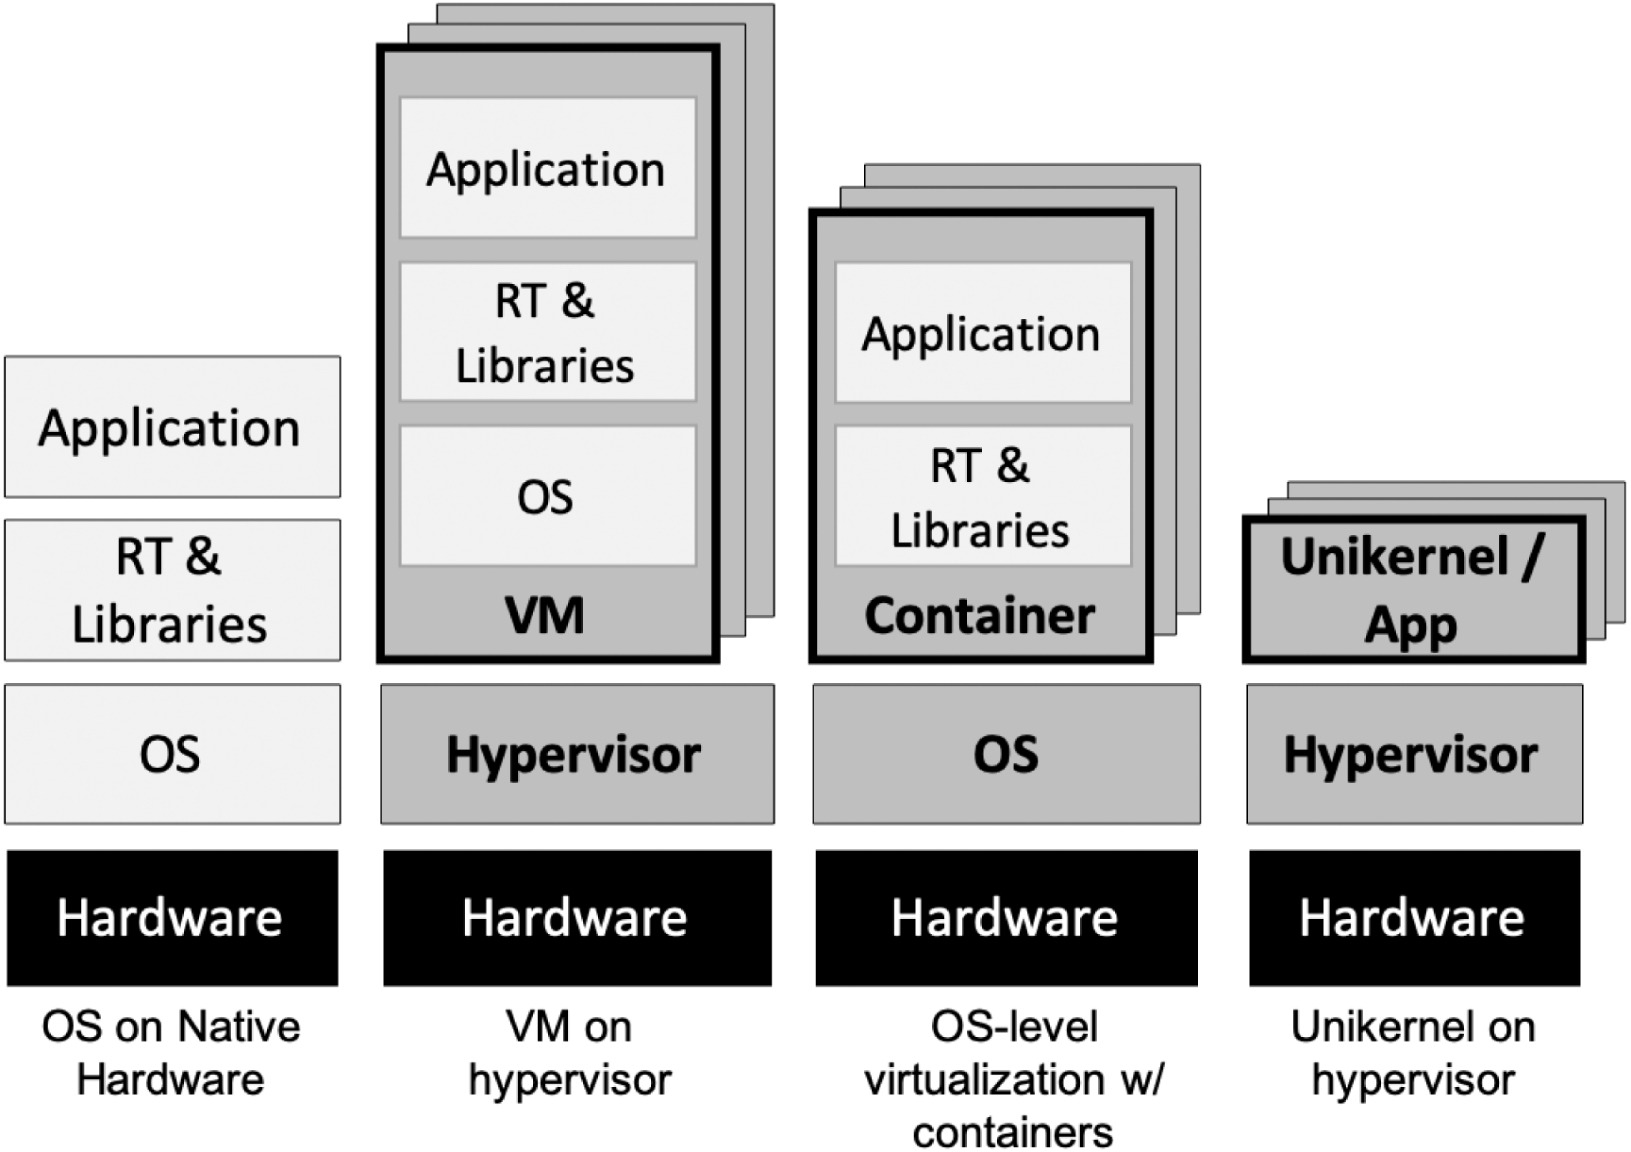
\includegraphics[width=0.6\textwidth]{./img/jpg/virt-approaches-exs} 
%  \includesvg[width=1.0\textwidth]{./img/virtualization.svg} 
  %\caption[Virtualization mind map]{Virtualization mind map}%
  \caption[Examples of virtualization approaches]{Examples of virtualization approaches~\cite{cinque2022virtualizing}\footnotemark}%
  \label{fig:virt-approaches-exs}
\end{figure}
%
\fnlicReq{Elsevier}{5457890117132}%
% \fnlicCCSA{foot:cc-lic}% CC licence

Cinque et.~al~\cite{cinque2022virtualizing} identified the relationship between hypervisor and guest
\gls{os} combinations, i.e.~the type of guest that runs on top of a hypervisor, and the
associated applications (Fig.~\ref{fig:virt-combos}).
On the left quadrants are represented the guest \glspl{os} running on top of a
general purpose hypervisor, mainly used for server consolidation in cloud
environments (bottom left), and functional testing and prototyping (top left).
On the right quadrants are represented the guest \glspl{os} on top of a \gls{rt}
hypervisor, mainly used for \gls{qos} and performance analysis (bottom right), and
safety-critical applications (top right). The region of interest -- the
\gls{mcs} -- is located in the intersection of these right quadrants,
emphasizing the need of a \gls{rt} hypervisor. Thus, the hypervisors will be
discussed in more detail in the next section.

\begin{figure}[!hbt]
  \centering
  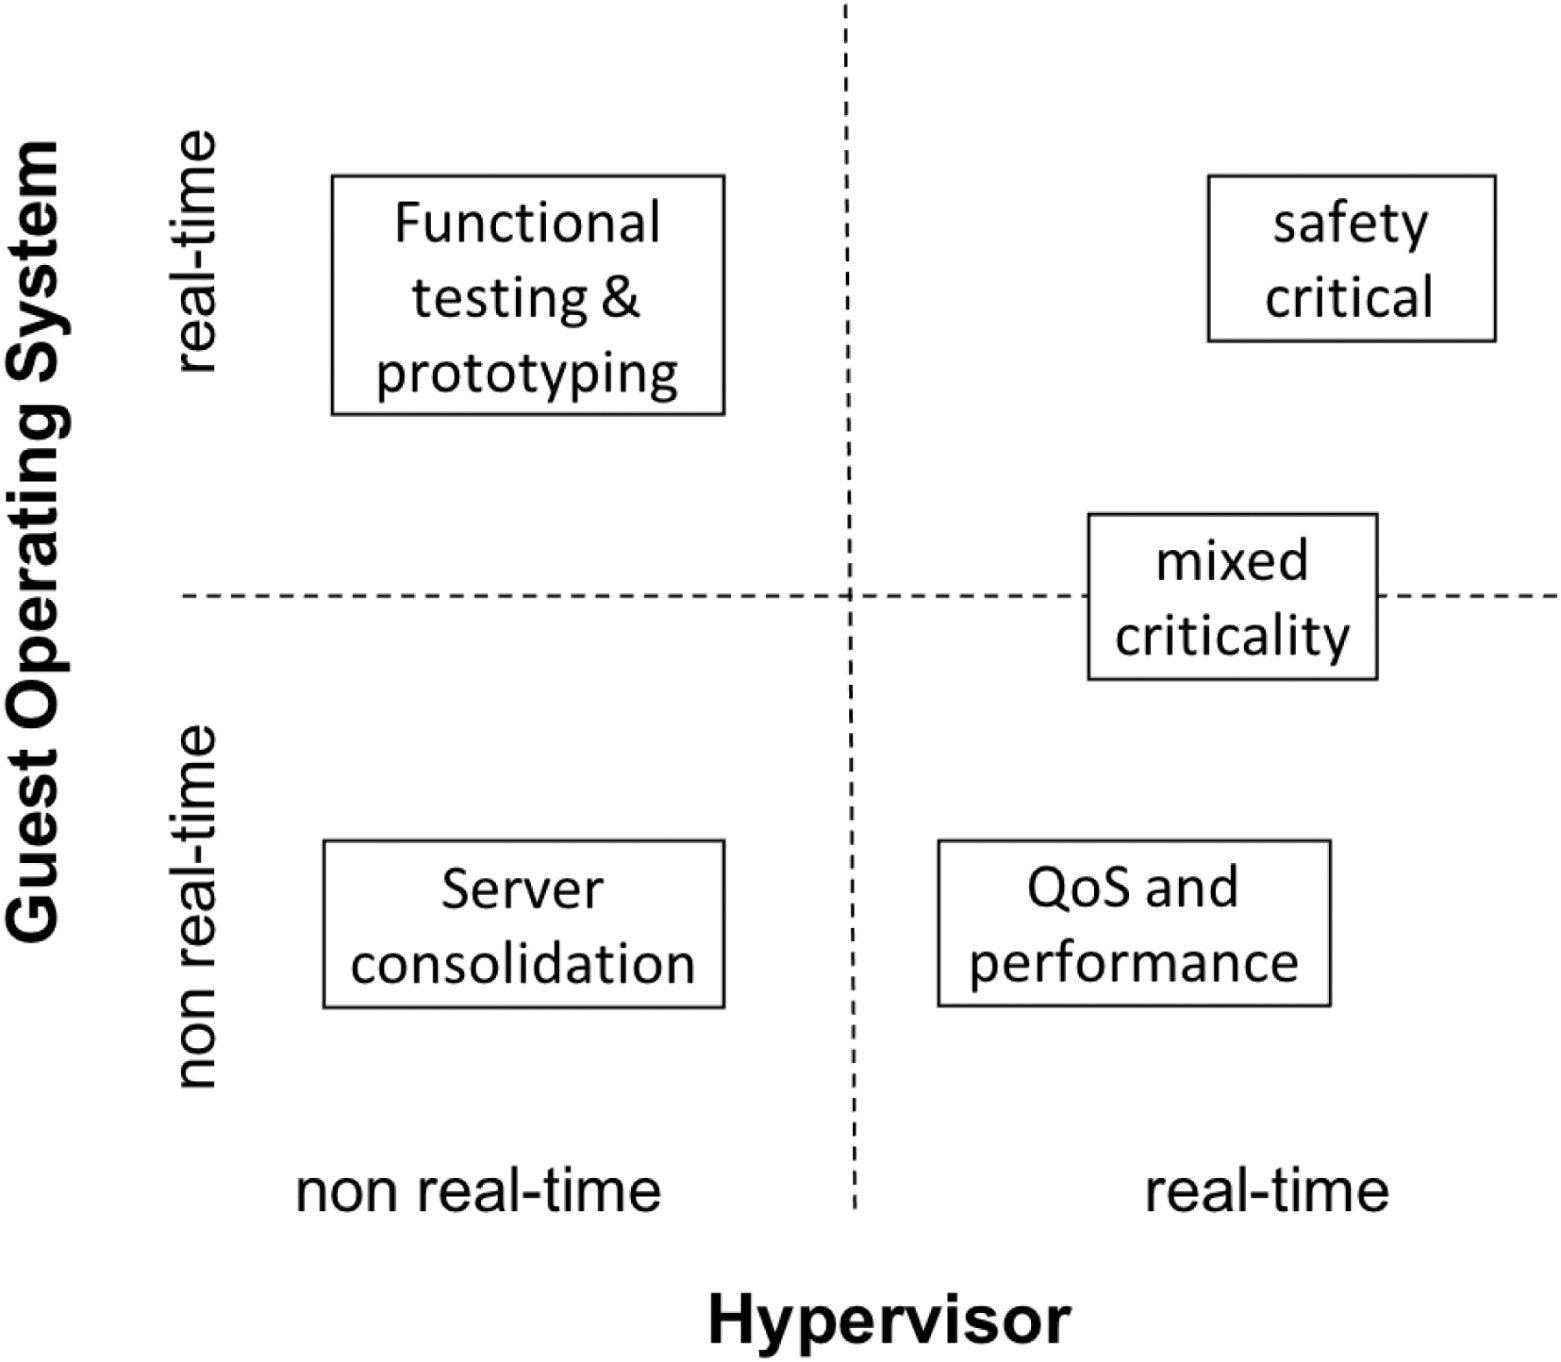
\includegraphics[width=0.6\textwidth]{./img/jpg/virt-combos} 
%  \includesvg[width=1.0\textwidth]{./img/virtualization.svg} 
  %\caption[Virtualization mind map]{Virtualization mind map}%
  \caption[Hypervisor and OS combinations with related applications]{Hypervisor
    and OS combinations with related applications~\cite{cinque2022virtualizing}\footnotemark}%
  \label{fig:virt-combos}
\end{figure}
%
\fnlicReq{Elsevier}{5457890117132}%
% \fnlicCCSA{foot:cc-lic}% CC licence

\subsection{Hypervisors}%
\label{sec:superv--hyperv}
In simple terms a hypervisor is a \glsxtrfull{vmm}, a software layer that
abstracts the \gls{hw} resources in order to run distinct and isolated
application environments, called \glspl{vm} or guests, on the same physical
machine (see Fig.~\ref{fig:virt-approaches-exs}). A \gls{vm} is the execution environment typically comprised of an
\gls{os}, or guest \gls{os}, and the application \gls{sw}.

A hypervisor must guarantee isolation in the following domains~\cite{cinque2022virtualizing}:
\begin{itemize}
\item \textbf{Temporal}:
  ability to isolate or limit the impact of resource consumption
  (e.g.~\gls{cpu}, network, disk) of a virtual domain on the performance degradation
  of other virtual domains. Thus, a task from one virtual domain must not cause serious
  delays to other tasks in other virtual domain. 
\item \textbf{Spatial} (memory-isolation): ability to isolate code and data
  between virtual domains and between virtual domains and hosts. Thus, a task
  must not be able to modify private data from other tasks, including devices
  assigned to a specific task. It is usually implementated using \gls{hw} memory
  protection mechanisms (e.g., \gls{mmu}, \gls{iommu}).
\item \textbf{Fault}: prevents the propagation of faults from one virtual domain
  to another that could cause blockages or stop the whole system.
\end{itemize}

A hypervisor can be classified in numerous ways (see
Fig.~\ref{fig:virt-mindmap}), as follows:
\begin{enumerate}
\item \textbf{Host presence}: If the hypervisor is executed on top of an
  existing \emph{host} \gls{os} --- \underline{hosted} --- is classified as type II,
  otherwise as type I --- \underline{bare-metal} ---, running directly on the \gls{hw},
  acting as a classic \gls{os}. The bare-metal hypervisor controls directly the
  hardware resources (e.g.~Jailhouse~\cite{jailhouse}, Bao~\cite{martins_et_al:OASIcs:2020:11779}), whereas the hosted manages it
  indirectly (e.g.~KVM~\cite{kivity2007kvm}, Xen).
\item \textbf{Guest awareness of the hypervisor}: A \underline{fully virtualized} hypervisor
  abstracts completely the \gls{hw} resources to the guest, emulating privileged
  instructions and \gls{io} operations. Thus, it allows a guest OS or an
  application to run unmodified, as they were running directly on the physical
  machine. Typical examples are KVM~\cite{kivity2007kvm} and Microsoft Hyper-V~\cite{microsoftHyperV}. Conversely, in a
  paravirtualized hypervisor (e.g., Xen~\cite{barham2003xen}) the guest \gls{os}
  must communicate with the underlying hypervisor through hypercalls, which is
  cumbersome, since it requires the guest \gls{os} to be modified.
\item \textbf{Real-time support}: this refers to the explicit support for the
  management of the time budget of each \gls{vm} (e.g.~scheduling algorithms)
  which must meet the explicit timing
  constraints~\cite{cinque2022virtualizing}. These hypervisors can be further
  decomposed in \underline{dynamic} (e.g.~KVM\cite{kivity2007kvm},
  Xen~\cite{barham2003xen}) or \underline{static} (e.g.~Jailhouse\cite{jailhouse}, Bao\cite{martins_et_al:OASIcs:2020:11779}), depending on the
  \gls{vm} resources assignment timing: in run-time, as needed, for the former;
  in instantiation time for the latter. Static solutions are often employed for
  \glspl{mcs} due to higher tolerance to failure and less overhead. Moreover, as
  they usually have a small code base they are easier to test and certify
  according to industrial standards~\cite{cinque2022virtualizing}.
\item \textbf{Application type}: embedded, if targeted for a specific application, system, or mission, otherwise they are general-purpose~\cite{heiser2008role}.
\end{enumerate}

Solutions based on hypervisors can be grouped in four categories~\cite{cinque2022virtualizing}:
\begin{enumerate}
\item \textbf{Separation kernel and microkernel}: specially designed for
  industrial and embedded domains. A separation kernel is a special type of a
  very small bare-metal hypervisor defining fixed \glspl{vm} and managing
  information flows, relegating device drivers, user model, shell access and
  dynamic memory to the guest \gls{os}. This simple architecture results in a
  minimal implementation, ideal for a \gls{mcs}. Examples are PikeOS~\cite{pikeOS}, Xtratum~\cite{masmano2009xtratum},
  Jailhouse~\cite{jailhouse}, and Bao~\cite{martins_et_al:OASIcs:2020:11779}.
\item \textbf{General-purpose}: enhancement of general-purpose hypervisors
  (e.g.~KVM~\cite{kivity2007kvm}, Xen~\cite{barham2003xen}) to
  support real-time features.
\item \textbf{Security \gls{cpu} \gls{hw} extensions}: leverage the isolation
  support provided by these hardware extensions (ARM TrustZone, Intel SGX) to attain stricter isolation
  guarantees. For example, ARM TrustZone eanbles virtual virtualization thanks
  to dual world execution model. However, these solutions are strictly linked to the specific
  platforms. Examples are LTZVisor/RTZVisor~\cite{pinto2016towards,rtzvisor} and VOSYSMonitor~\cite{vosysmonitor,lucas2017vosysmonitor}.%
\item \textbf{Unikernel}: runs on top of an hypervisor to enable the execution
  of a single application in its virtual domain, providing isolation,
  performance, and security. Examples are ClickOS~\cite{martins2014clickos} and HermitCore~\cite{lankes2016hermitcore}.
\end{enumerate}

The selection factors for a hypervisor with industrial standards are its footprint, the compliance with
industry safety-related standard, the software license, the explicit support to
high availability, fault tolerance and security, and the supported \gls{hw}
platform~\cite{cinque2022virtualizing}. Cinque et.~al provides an extensive list
of these solutions applied to the \gls{mcs} in order to meet the industrial standards~\cite{cinque2022virtualizing}.

\subsubsection{Bao}%
\label{sec:bao}


Bao (from Mandarin Chinese ``bǎohù'', meaning ``to protect'') is a security and
safety-oriented, lightweight bare-metal hypervisor, developed by the ESRGv3 team
at University of Minho, targeting the embedded real-time domain and especially
the \glspl{mcs} for Armv8 and RISC-V platforms. It follows the pioneer static partioning architecture of
\emph{Jailhouse}~\cite{jailhouse}, and improves it by discarding the need of the
Linux Kernel to boot and manage its \glspl{vm}. From a security and
safety perspective, this dependency compromises the system by bloating the
system \gls{tcb} and intercepting the chain of trust in secure boot
mechanisms~\cite{martins_et_al:OASIcs:2020:11779}. The \glspl{mcs} certification
process is also hindered by the size of and monolithic architecture of such \glspl{os}.

\emph{Jailhouse}'s breakthrough consists in a minimal software layer that
leverages \gls{hw}-assisted virtualization technology to
statically partition all platform resources and assign each one exclusively to a
single \gls{vm} instance at instantiation time. The scheduler can then be
discarded as each virtual core is statically associated to a single physical
CPU, and the complex semantic services are relegated for the \glspl{vm}, further
decreasing the size and complexity. It provides strong isolation and real-time
guarantees but at the expense of efficient resource usage requirement. However,
the Linux dependency is a liability for safety/security and performance too.

Furthermore, the static partioning approach is not enough \emph{per se}, due to
\gls{hw} resources sharing across partitions such as \glspl{llc}, interconnects,
and memory controllers, which breach temporal isolation, hurting performance and
determinism~\cite{bansal2018evaluating,barham2003xen}. A malicious \gls{vm} can exploit this by increasing their
usage of a share resource (\gls{dos} attack) or by indirectly accessing other
gls{vm}'s data thorugh the implicit timing side-channels~\cite{ge2018survey}. To tackle this
issue, some techniques were implemented at both the OS and hypervisor level such
as cache partioning (via locking or coloring), and memory bandwidth
reservations~\cite{martins_et_al:OASIcs:2020:11779}.

Taking this into account Bao was implemented as clean-slate
hypervisor (see Fig.~\ref{fig:bao-arch}), comprising only a minimal thin layer of privileged \gls{sw}
leveraging \gls{isa} virtualization support to implement static partioning of
\gls{hw} resources. Its most relevant features are: memory is statically
assigned using 2-stage translation; \gls{io} is pass-through only; 1:1 mapping
of virtual to physical \glspl{cpu} (no scheduler required); no external
dependencies (except for standard platform management \gls{sw}); provides a
basic mecanism for inter-\gls{vm} communication; \gls{tee} support for increased
security~\cite{martins_et_al:OASIcs:2020:11779,baoEmbeddedWorld2020}.

\begin{figure}[!hbt]
  \centering
  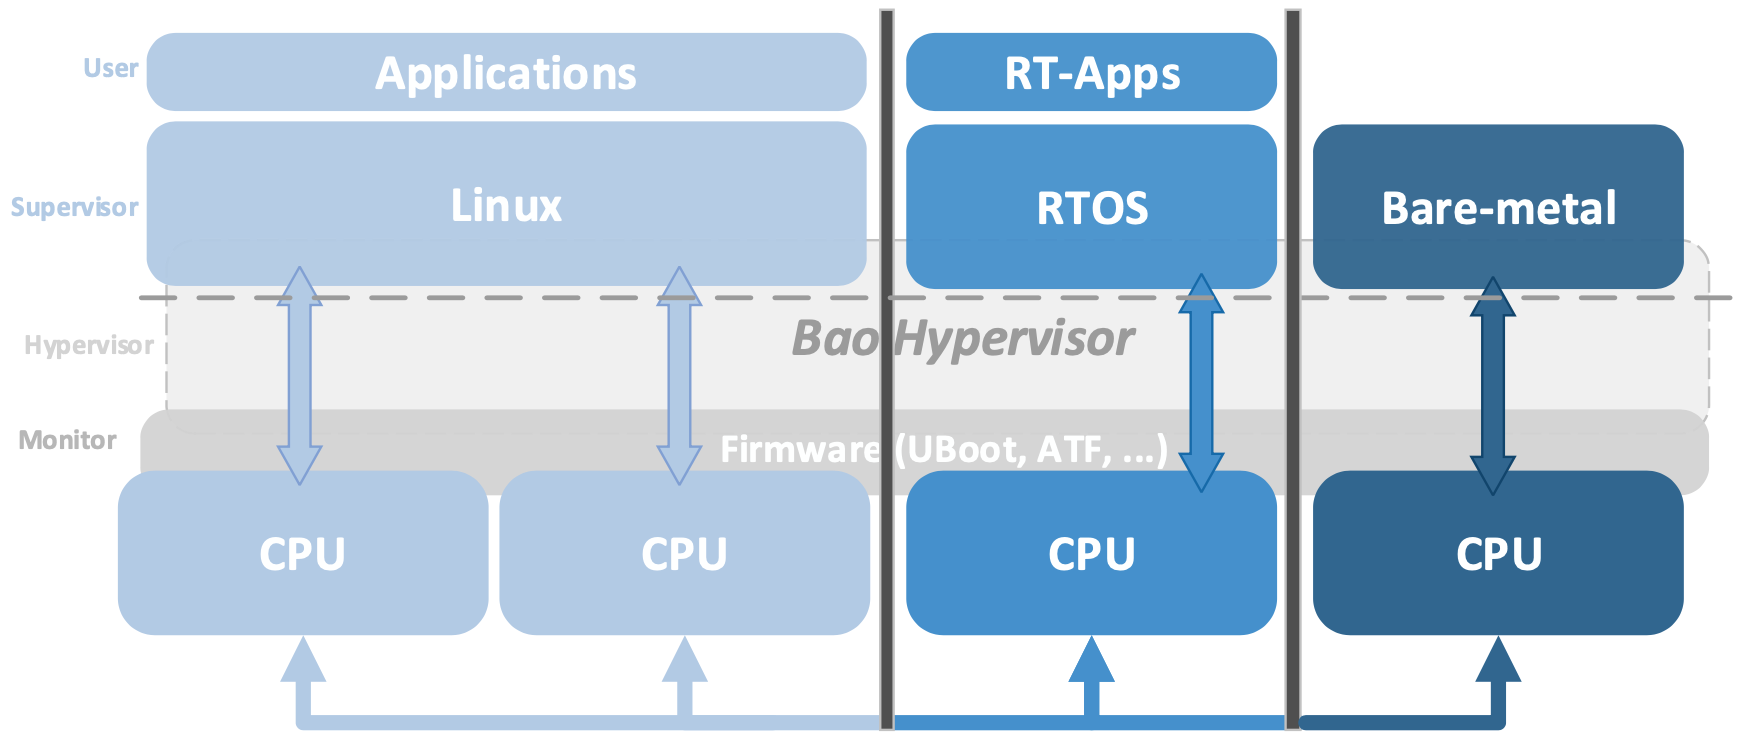
\includegraphics[width=0.7\textwidth]{./img/png/bao-arch} 
%  \includesvg[width=1.0\textwidth]{./img/virtualization.svg} 
  %\caption[Virtualization mind map]{Virtualization mind map}%
  \caption[Hypervisor Bao architecture]{Hypervisor Bao architecture~\cite{martins_et_al:OASIcs:2020:11779}\footnotemark}%
  \label{fig:bao-arch}
\end{figure}
%
%\fnlicReq{Elsevier}{5457890117132}%
\fnlicCC{foot:bao-embedded-world-lic1}%

Guest isolation is critical for a \gls{mcs}. Bao achieves complete logical
temporal isolation due to the exclusive CPU mapping, discarding the scheduler,
and the availability of per-\gls{cpu} architectural timers directly managed by
the guests. Spatial isolation is provided by the 2-stage \gls{hw} virtualization
support for the logical address space isolation. The translation overhead, page
table and \gls{tlb} pressure is minimized using superpages, whenever
possible, faciliting speculative fetch for potential guest performance
improvement. A page coloring mechanism was implemented to enable \gls{llc}
cache partioning independently for each \gls{vm}, but at the expenses of memory
waste and fragmentation, and increased boot time~\cite{martins_et_al:OASIcs:2020:11779}.

The \gls{io} are directly assigned to guests in a pass-through only
configuration. For the memory-mapped IO architectures, as the ones supported, it
uses the existing memory mechanism and 2-stage translation provided by the
virtualization support to implement this for free. A peripheric can be shared
among guests, as exclusive assignment is not checked~\cite{martins_et_al:OASIcs:2020:11779}.

The interrupt virtualization support is restricted to the Arm \gls{gic}v2 and
Arm \gls{gic}v3, which does not support direct interrupt delivery to guest
partitions. Instead, all interrupts
are dispatched to the hypervisor, which then must re-inject them into the guest \gls{vm} using
a limited set of pending registers, leading to unavoidable increase in both
interrupt latency and the complexity of interrupt management code~\cite{martins_et_al:OASIcs:2020:11779}. This was
fixed in the newest version of the specification~\gls{gic}v4 which bypasses the hypervisor for guest interrupt delivery~\cite{dall2018design}.

It is also noteworthy to mention that Xen has recently introduced
\emph{Dom0-less}, eliminating the Linux dependency to boot and execute its
hypervisor and \glspl{vm}. Nonetheless, Bao currently provides the same
features but with a smaller \gls{tcb} and with clean security
features. Moreover, and although being in its infancy, preliminary evaluation
demonstrate only minimal virtualization overhead~\cite{martins_et_al:OASIcs:2020:11779}.
Lastly, Bao is open-source~\cite{baoRepo} due to the developing team's strong
belief that security requires transparency. For all the aforementioned reasons,
Bao is the hypervisor of choice to use in this work. Tab.~\ref{tab:bao-summary}
provides a summary of the Bao hypervisor.

% Please add the following required packages to your document preamble:
% \usepackage{multirow}
% \usepackage{graphicx}
% \usepackage[table,xcdraw]{xcolor}
% If you use beamer only pass "xcolor=table" option, i.e. \documentclass[xcolor=table]{beamer}
\begin{table}[]
\centering
\caption{Bao hypervisor summary}%
\label{tab:bao-summary}
\resizebox{\textwidth}{!}{%
\begin{tabular}{lllll}
\hline
{\color[HTML]{000000} \textbf{Architecture}} &
  {\color[HTML]{000000} \textbf{Supported platforms}} &
  {\color[HTML]{000000} \textbf{Size}} &
  {\color[HTML]{000000} \textbf{License}} &
  {\color[HTML]{000000} \textbf{Version}} \\ \hline
{\color[HTML]{000000} \begin{tabular}[c]{@{}l@{}}Type I,\\ Static\end{tabular}} &
  {\color[HTML]{000000} \begin{tabular}[c]{@{}l@{}}Armv8\\ RISC-V (experimental)\end{tabular}} &
  {\color[HTML]{000000} \begin{tabular}[c]{@{}l@{}}Small \\ $\sim$5 kLOC C + $\sim$500 LOC ASM\end{tabular}} &
  {\color[HTML]{000000} GPLv2} &
  {\color[HTML]{000000} 0.1.1.} \\ \hline
{\color[HTML]{000000} \textbf{Features}} &
  \multicolumn{4}{c}{{\color[HTML]{000000} \textbf{Isolation}}} \\ \hline
{\color[HTML]{000000} Static partioning} &
  \multicolumn{2}{l}{{\color[HTML]{000000} \textbf{Spatial}}} &
  \multicolumn{2}{l}{{\color[HTML]{000000} \textbf{Temporal}}} \\ \cline{2-5} 
{\color[HTML]{000000} IO pass-thorugh only} &
  \multicolumn{2}{l}{{\color[HTML]{000000} }} &
  \multicolumn{2}{l}{{\color[HTML]{000000} }} \\
{\color[HTML]{000000} \begin{tabular}[c]{@{}l@{}}1:1 mapping of virtual to physical CPUs \\ (no scheduler required)\end{tabular}} &
  \multicolumn{2}{l}{\multirow{-2}{*}{{\color[HTML]{000000} \begin{tabular}[c]{@{}l@{}}Provided by a 2-stage translation \\ HW virtualization support\end{tabular}}}} &
  \multicolumn{2}{l}{\multirow{-2}{*}{{\color[HTML]{000000} \begin{tabular}[c]{@{}l@{}}Exclusive CPU assignment \\ discards the scheduler\end{tabular}}}} \\
{\color[HTML]{000000} Virtual interrupts directly mapped to physical ones} &
  \multicolumn{2}{l}{{\color[HTML]{000000} }} &
  \multicolumn{2}{l}{{\color[HTML]{000000} }} \\
 &
  \multicolumn{2}{l}{{\color[HTML]{000000} }} &
  \multicolumn{2}{l}{{\color[HTML]{000000} }} \\
 &
  \multicolumn{2}{l}{{\color[HTML]{000000} }} &
  \multicolumn{2}{l}{{\color[HTML]{000000} }} \\
\multirow{-3}{*}{\begin{tabular}[c]{@{}l@{}}No external dependencies (except for standard \\ platform management firmware)\end{tabular}} &
  \multicolumn{2}{l}{\multirow{-4}{*}{{\color[HTML]{000000} \begin{tabular}[c]{@{}l@{}}Translation overhead is minimized using superpages \\ whenever possible, faciliting speculative fetch \\ for potential guest performance improvement\end{tabular}}}} &
  \multicolumn{2}{l}{{\color[HTML]{000000} }} \\
{\color[HTML]{000000} } &
  \multicolumn{2}{l}{{\color[HTML]{000000} }} &
  \multicolumn{2}{l}{{\color[HTML]{000000} }} \\
\multirow{-2}{*}{{\color[HTML]{000000} \begin{tabular}[c]{@{}l@{}}Provides a basic mecanism for inter-VM \\ communication\end{tabular}}} &
  \multicolumn{2}{l}{{\color[HTML]{000000} }} &
  \multicolumn{2}{l}{{\color[HTML]{000000} }} \\
{\color[HTML]{000000} } &
  \multicolumn{2}{l}{{\color[HTML]{000000} }} &
  \multicolumn{2}{l}{{\color[HTML]{000000} }} \\
\multirow{-2}{*}{{\color[HTML]{000000} \begin{tabular}[c]{@{}l@{}}Trusted Execution Environment support \\ for increased security\end{tabular}}} &
  \multicolumn{2}{l}{{\color[HTML]{000000} }} &
  \multicolumn{2}{l}{{\color[HTML]{000000} }} \\
{\color[HTML]{000000} } &
  \multicolumn{2}{l}{{\color[HTML]{000000} }} &
  \multicolumn{2}{l}{{\color[HTML]{000000} }} \\
\multirow{-2}{*}{{\color[HTML]{000000} \begin{tabular}[c]{@{}l@{}}State-of the art partioning mechanisms to be \\ implemented (e.g., memory throttling)\end{tabular}}} &
  \multicolumn{2}{l}{\multirow{-6}{*}{{\color[HTML]{000000} \begin{tabular}[c]{@{}l@{}}It uses cache coloring to enable LLC cache \\ partioning independently for each VM, but at \\ the expenses of memory waste and fragmentation \\ and increased boot time\end{tabular}}}} &
  \multicolumn{2}{l}{\multirow{-10}{*}{{\color[HTML]{000000} \begin{tabular}[c]{@{}l@{}}Per-CPU architecture timers \\ are available to and directly \\ managed by the guests\end{tabular}}}} \\ \hline
{\color[HTML]{000000} \textbf{IO}} &
  \multicolumn{2}{l}{{\color[HTML]{000000} \textbf{Interrupts}}} &
  \multicolumn{2}{l}{{\color[HTML]{000000} \textbf{Related Work}}} \\ \hline
{\color[HTML]{000000} } &
  \multicolumn{2}{l}{{\color[HTML]{000000} }} &
  \multicolumn{2}{l}{{\color[HTML]{000000} }} \\
{\color[HTML]{000000} } &
  \multicolumn{2}{l}{{\color[HTML]{000000} }} &
  \multicolumn{2}{l}{{\color[HTML]{000000} }} \\
\multirow{-3}{*}{{\color[HTML]{000000} \begin{tabular}[c]{@{}l@{}}Directly assigned to guest in a \\ pass-through only IO configuration\end{tabular}}} &
  \multicolumn{2}{l}{\multirow{-3}{*}{{\color[HTML]{000000} Currently supports only Arm GICv2}}} &
  \multicolumn{2}{l}{\multirow{-3}{*}{{\color[HTML]{000000} \begin{tabular}[c]{@{}l@{}}Jailhouse: pioneer in the static \\ partioning adopted by Bao but \\ requires the Linux Kernel to boot\end{tabular}}}} \\
{\color[HTML]{000000} } &
  \multicolumn{2}{l}{{\color[HTML]{000000} }} &
  \multicolumn{2}{l}{{\color[HTML]{000000} }} \\
{\color[HTML]{000000} } &
  \multicolumn{2}{l}{{\color[HTML]{000000} }} &
  \multicolumn{2}{l}{{\color[HTML]{000000} }} \\
{\color[HTML]{000000} } &
  \multicolumn{2}{l}{{\color[HTML]{000000} }} &
  \multicolumn{2}{l}{{\color[HTML]{000000} }} \\
{\color[HTML]{000000} } &
  \multicolumn{2}{l}{{\color[HTML]{000000} }} &
  \multicolumn{2}{l}{{\color[HTML]{000000} }} \\
\multirow{-5}{*}{{\color[HTML]{000000} \begin{tabular}[c]{@{}l@{}}For memory-mapped IO it uses the existing \\ memory mechanism and 2-stage translation \\ provided by the virtualization support\end{tabular}}} &
  \multicolumn{2}{l}{\multirow{-5}{*}{{\color[HTML]{000000} \begin{tabular}[c]{@{}l@{}}Interrupts are forwarded to the hypervisor which \\ must re-inject them in the VM using a limited set \\ of pending registers\end{tabular}}}} &
  \multicolumn{2}{l}{\multirow{-5}{*}{{\color[HTML]{000000} \begin{tabular}[c]{@{}l@{}}Xen Dom0-less: eliminates the \\ Linux dependency to boot and \\ execute\end{tabular}}}} \\
{\color[HTML]{000000} } &
  \multicolumn{2}{l}{{\color[HTML]{000000} }} &
  \multicolumn{2}{l}{{\color[HTML]{000000} }} \\
{\color[HTML]{000000} } &
  \multicolumn{2}{l}{{\color[HTML]{000000} }} &
  \multicolumn{2}{l}{{\color[HTML]{000000} }} \\
{\color[HTML]{000000} } &
  \multicolumn{2}{l}{{\color[HTML]{000000} }} &
  \multicolumn{2}{l}{{\color[HTML]{000000} }} \\
{\color[HTML]{000000} } &
  \multicolumn{2}{l}{{\color[HTML]{000000} }} &
  \multicolumn{2}{l}{{\color[HTML]{000000} }} \\
\multirow{-5}{*}{{\color[HTML]{000000} \begin{tabular}[c]{@{}l@{}}A peripheric can be shared among guests \\ (exclusive assignment is not checked)\end{tabular}}} &
  \multicolumn{2}{l}{\multirow{-5}{*}{{\color[HTML]{000000} \begin{tabular}[c]{@{}l@{}}Fixed in GICv4 which bypasses the hypervisor for \\ guest interrupt delivery\end{tabular}}}} &
  \multicolumn{2}{l}{\multirow{-5}{*}{{\color[HTML]{000000} \begin{tabular}[c]{@{}l@{}}Bao provides the same features \\ from the previous ones, but has \\ a smaller TCB and implements \\ clean security features\end{tabular}}}} \\ \hline
\end{tabular}%
}
\end{table}

\section{Unmanned Aerial Vehicles}%
\label{sec:unmann-aeri-vehicl}
\glsxtrfull{uav}s, \glsxtrfull{uas}, or more commonly drones, are a class of
unmanned robotic vehicles that can execute flying missions and carry payloads,
guided either by remote control stations or in an autonomous
way~\cite{alladi2022UAVBlockain,glossner2021overview}.
They belong to a broader class of \glspl{uv}, alongside with \glspl{ugv}, \glspl{usv}
(e.g., boats) and \glspl{uuv}~\cite{glossner2021overview}.

\glspl{uav} date back to as far as the 18\textsuperscript{th} century. In 1783,
France, the first uncrewed aircraft --- a hot air balloon ---
was publicly displayed~\cite{Blundell2020,alladi2022UAVBlockain}. In 1896, Alfred Nobel created the first camera-based \gls{uav}
(rocket) and launched it. In 1935, U.K., the first modern \gls{uav} was
developed, a low cost radio controlled aircraft. The term \emph{drone} was
presumably coined by Lieutenant Commander Fahrney, who as in charge of U.S. Navy
program \emph{Radio Controlled Aircraft}~\cite{Blundell2020}. The first \gls{uav} designed for
surveillance and scouting was developed in 1973 in Israel, and the \emph{Gulf
  War} was the first conflict utilizing \glspl{uav}. Starting from 2003,
the \gls{uav} commercial market started to emerge with the release of the
\emph{Amazon Prime}~~\cite{alladi2022UAVBlockain}.
However, it was until 2006 that the \glspl{uav} were first
permitted in the U.S. civilian space. More recently, in 2010, the first
smartphone controlled quadcopter was developed, and in 2013 camera equipped
\glspl{uav} entered the consumer market~\cite{uavHistory}.

From then on, the selling price dropped significantly, alongside with the
emergence of some of the first open-source projects on \gls{uav} control ---
ArduPilot in 2008~\cite{arduPilotHistory} and Dronecode~\cite{px4History} (now PX4) in 2011 --- led to a boom in the
commercial \gls{uav} market. In 2017 the North America market had a revenue of
737 million USD dollars and a eight-fold increase is expected for 2026 with a
staggering 6.7 billion USD dollars, with strong contributions from the sectors
of agriculture and farming, and security and law enforcement~\cite{mohsan2022towards}.

The versatility and utility of \glspl{uav} are well displayed is by its wide
range of applications, performing tasks with high added value and that would be
somewhat hard or impossible for a person to achieve: rescue operations and
saving lifes, agriculture and farming, building structures, pipeline
inspections, delivering goods and medical supplies, video capturing and filming,
surveying, inventory management, providing telecommunications in remote areas,
among others~\cite{alladi2022UAVBlockain}.

However, only recently regulations have been explicitly enforced on \glspl{uav},
with many countries allowing drones to fly over populated areas (at altitudes
lower than 150 m)~\cite{nassi2021sok}. For example, in 2019, the E.U.~stated that all drones under
25 kgs are able to fly without prior authorization under some constraints. On
the other hand, it imposed that all drones must register in their respective
states, and that each state must define no-fly zones where drones are
forbidden to enter~\cite{Ullah2020UAV5gEULegisl}. Broadly, five important categories must be considered when
analyzing the \gls{uav}
regulations~\cite{fotouhi2019UAVCellularCommSurvey,stocker2017UAVRegulationsReview}:

\begin{enumerate}
\item \textbf{Applicability}: refers to the applicable scope of \gls{uav} regulations,
  typically including type, weight, and role of the \gls{uav}; 
\item \textbf{Operational limitations}: restricts the locations for \gls{uav} operations.
\item \textbf{Administrative and legal requirements}: set of rules and
  regulations to monitor the use of \glspl{uav}.
\item \textbf{Technology specifications/requirements}: mechanical,
  communications and control capabilities that ensure its safe operation.
\item \textbf{Moral and ethics}: refers to the privacy and security of people in
  general.
\end{enumerate}

Furthermore, no global regulation for \gls{uav} standardization exists. Thus, in
2020 \gls{faa} in collaboration with \gls{nasa} and other agencies published the
\gls{utm} 2.0, describing protocols for enabling multiple, \gls{bvlos}
drone operations with the same airspace.

\subsection{Classification}%
\label{sec:classification}
An \gls{uav} can be classified in multiple ways:
\begin{itemize}
\item \textbf{Thrust forces \& Flight principles}: \glspl{uav} can be lighter
  than air, e.g., a balloon or a blimp if it uses a motorized propulsion
  system. On the other hand, if they are heavier than air, they are named
  gliders, rotor-crafts, and birds~\cite{mohsan2022towards}.
 % 
\item \textbf{Airframe}: probably the most noticeable external feature of a
  \gls{uav} is its chassis, or airframe. Several airframes exist for different
  applications from three main types: fixed-wing, rotor, and
  hybrid. Fixed-wing can travel faster than all other types of \glspl{uav} due
  to its aerodynamics and propulsion system, can carry heavy payloads, and have
  long autonomy. However, they require takeoff and landing from a runway. They
  are typically used for power line inspections and aerial mapping. Single rotor
  and multirotor \gls{uav} can hover and do \gls{vtol}. The single rotor long
  autonomy, but are expensive, require skilled operators, and are mechanically
  complex and vulnerable to vibrations. Multirotors, on the other hand, are the
  cheapest and most manufactured ones, but they typically have low autonomy
  since they consume more power. They can have a varied number of propelers,
  such as tricopter, quadcopter, hexacopter, and octocopter~\cite{mohsan2022towards}.
 % 
\item \textbf{Altitude}: Broadly, \glspl{uav} are divided into \glspl{lap} and
  \glspl{hap}~. A \gls{lap} maximum altitude ranges from 3 to 9 kms and is
  typically used to support cellular communications. \glspl{hap}, on the other
  hand, are deployed above the 9 km altitude and are used to support cellular
  communication but with wider coverage, endorsed by companies such as Google
  and Facebook~\cite{mohsan2022towards}.
%  
\item \textbf{Overall weight}: \glspl{uav} can have few grams of weight or
  hundreds of kilograms. For example, Australia labels them as \emph{micro}
  (below 100 g),
  \emph{very small} (from 100 g to 2 kg), \textbf{small} (from 2 to 25 kgs),
  \textbf{medium} (from 25 to 150 kgs), and \textbf{large} (over
  150 kgs)~\cite{alladi2022UAVBlockain}.
%  
\item \textbf{Power source}: \glspl{uav} can be powered using electricity,
  fuel, or a hybrid solution. Except for the fuel-only powered ones (e.g., Nitro
  Stingray, and Goliath Quadcopter~\cite{gasPoweredDrone}), all the
  others use electric motors. These motors can be powered through batteries
  (e.g., Parrot\cite{parrotDrone}, Dji Mavic 3~\cite{djiMavic3Drone}),
  typically \gls{lipo}, \glspl{hfc} (e.g., Energyor H2Quad 1000~\cite{energyorDrone}), and solar power. The
  hybrid solutions use fuel + batteries (e.g., Flaperon MX8~\cite{flaperonDrone}) or \gls{hfc} + batteries, and are a compromise between the
  two power sources. Batteries typically have the shortest autonomy and are
  heavy and bulky, while fuel, although not a clean power source, has the
  highest power density, leading to higher autonomy. The hydrogen fuel cells are
  a intermediate solution, but are typically more expensive than batteries and
  have more complex power management.
%  
\item \textbf{Target audience}: \glspl{uav} are developed with a specific target
  audience in mind, namely the recreational/hobbyist, the commercial, and
  military one.
%  
\item \textbf{User-modifiable}: In 2021, 26\% of all commercial drones sold were
  open-source (e.g., Parrot)~\cite{droneAnalyst2021}. There is an increased trend for open-source
  adoption due to higher transparency, extensability and usage from the end-user
  perspective, and due to bootstrapping opportunity since the developers can
  leverage from the ecosystem, e.g., using the flight control algorithms which
  are hard and costly to develop.
  At the other end of the spectrum lie proprietary drones (e.g., Dji), which hold the highest market share.
  Transparency is
  compromised and extensibility is typically provided using a \gls{sdk}~\cite{djiSDK}.
\end{itemize}

Fig.~\ref{fig:uav-types} illustrates the several types of \glspl{uav}, focusing
on airframe and power source. 
The most prominent \gls{uav}'s characteristics are speed, autonomy, payload,
range, and altitude. The speed depends mainly on the propulsion system,
aerodynamics, weather conditions and power usage. Typically, a small
\gls{uav} can reach speeds up to 50 km/h, while a large one can reach speeds up
to 360 km/h\cite{mohsan2022towards}.

% UAV TYPES
\begin{figure}[htb!]
  \centering
  %
  \begin{subfigure}[t]{0.35\textwidth}
  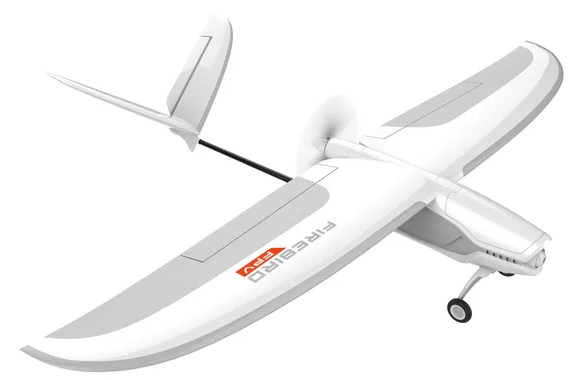
\includegraphics[width=1.0\textwidth]{./img/png/uav-FirebirdFPV-FixedWing.png}
  \caption{Firebird: Fixed-wing~\cite{firebirdDrone}}%
  \label{fig:uav-fixed-wing}
  \end{subfigure}
%
  \begin{subfigure}[t]{0.35\textwidth}
  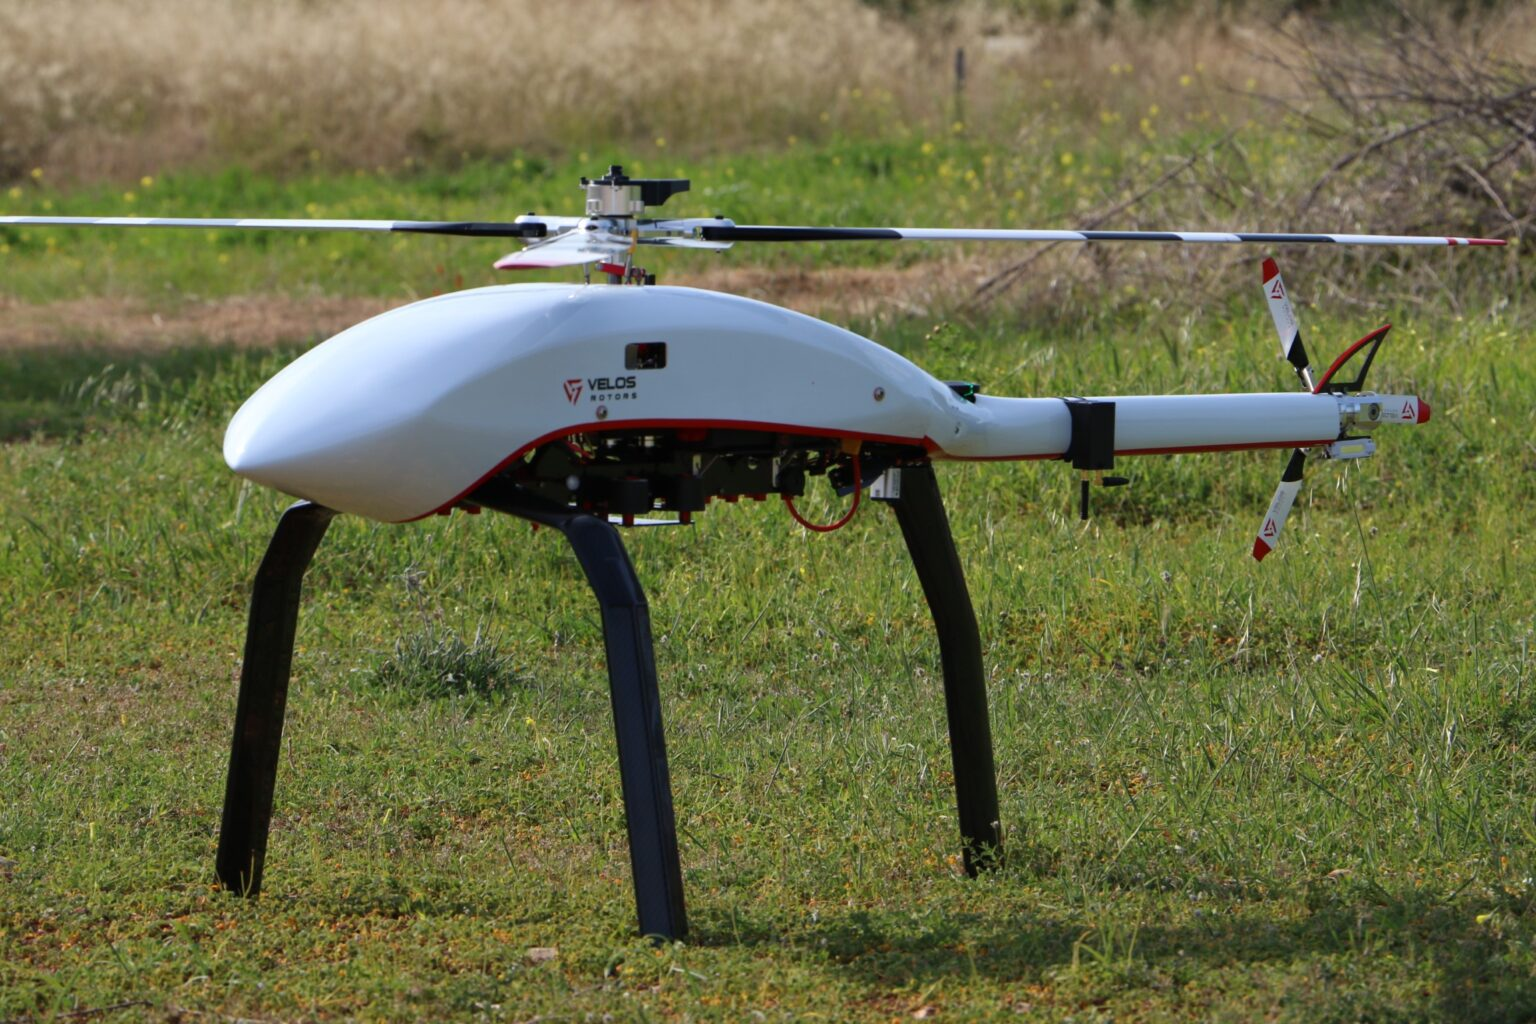
\includegraphics[width=1.0\textwidth]{./img/jpg/uav-velos-singleRotor.jpg}
  \caption{Velos: single-rotor~\cite{velosDrone}}%
  \label{fig:uav-single-rotor}
\end{subfigure}

  \begin{subfigure}[t]{0.35\textwidth}
  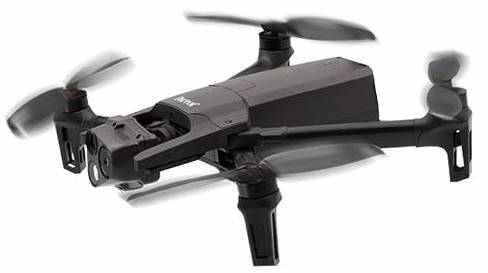
\includegraphics[width=1.0\textwidth]{./img/jpg/uav-parrot-multirotor.jpg}
  \caption{Parrot: multirotor~\cite{parrotDrone}}%
  \label{fig:uav-multirotor}
  \end{subfigure}
%
  \begin{subfigure}[t]{0.35\textwidth}
  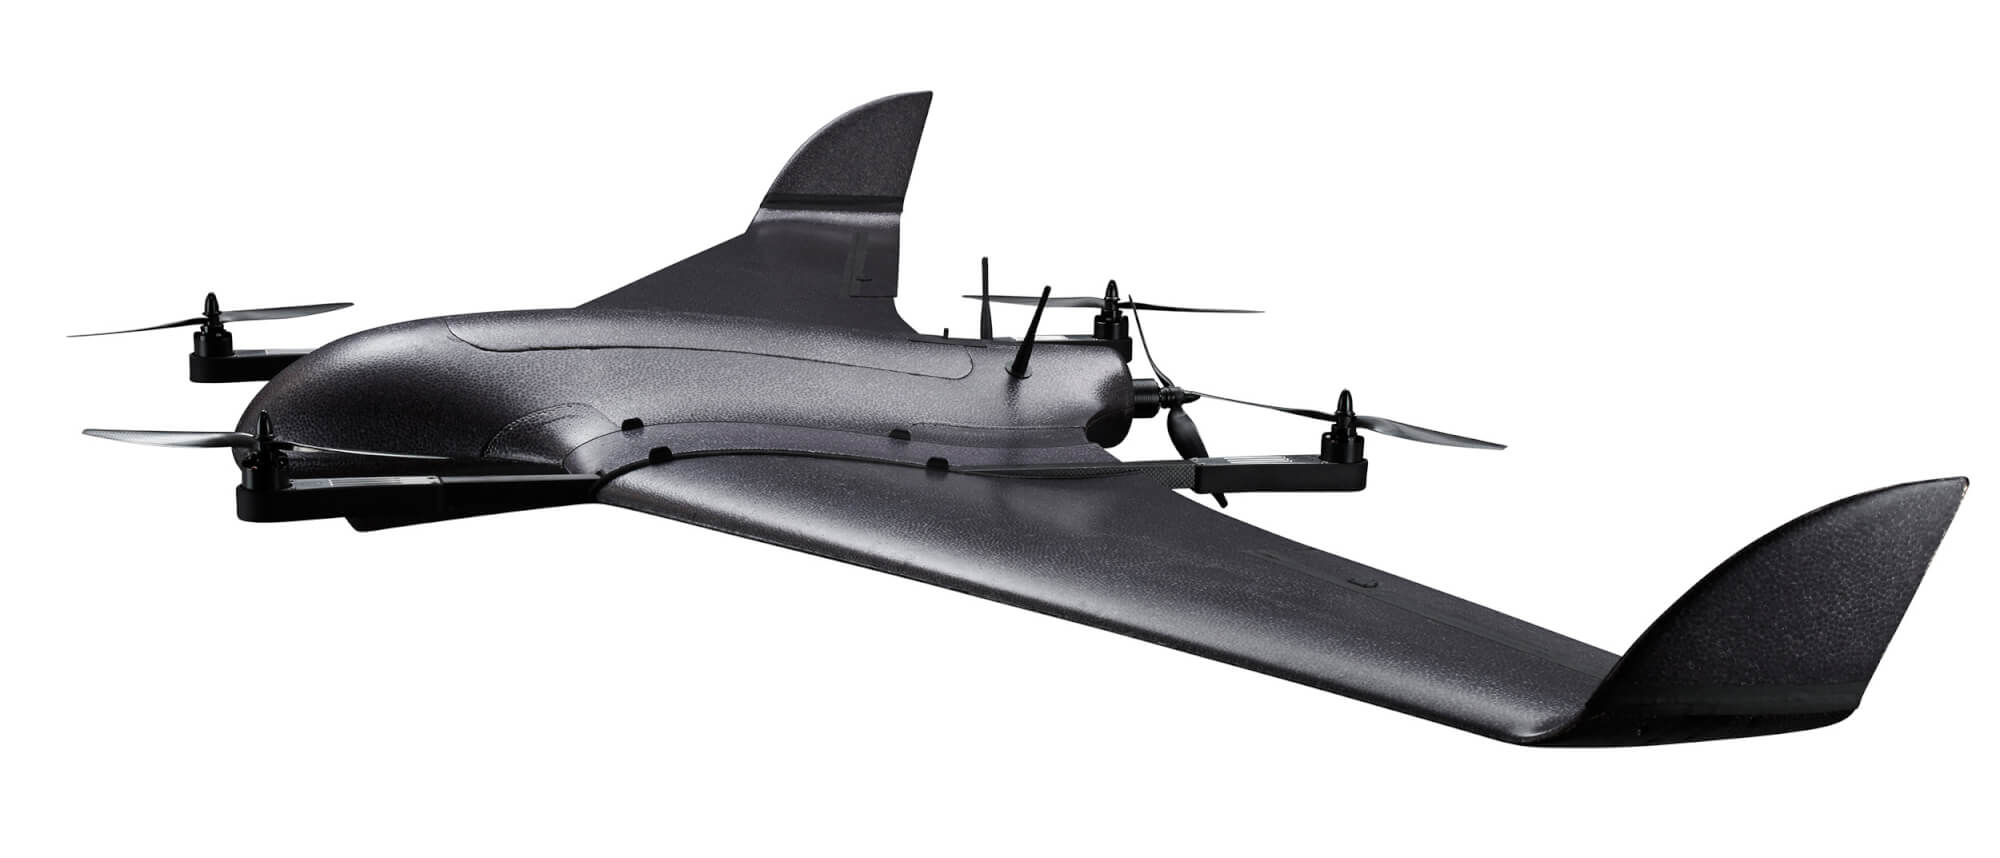
\includegraphics[width=1.0\textwidth]{./img/jpg/uav-deltaQuadPro-hybrid.jpg}
  \caption{DeltaQuad Pro: fixed-wing hybrid~\cite{deltaQuadDrone}}%
  \label{fig:uav-fixed-wing-hybrid}
  \end{subfigure}
%
  \begin{subfigure}[t]{0.35\textwidth}
  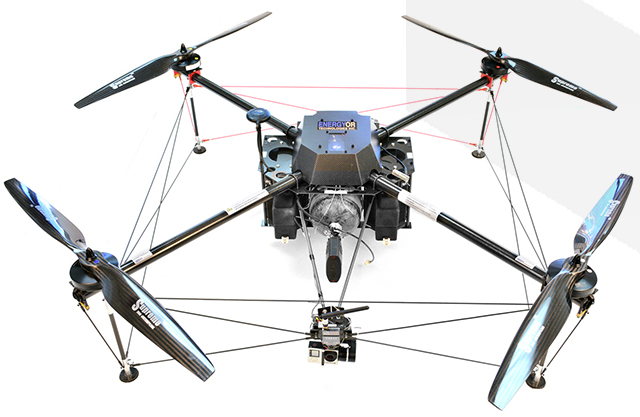
\includegraphics[width=1.0\textwidth]{./img/jpg/uav-energyorQuad1000-hfc.jpg}
  \caption{Energyor Quad 1000: hybrid (HFC + batteries)~\cite{energyorDrone}}%
  \label{fig:uav-energyor-hfc}
  \end{subfigure}
  % 
  \begin{subfigure}[t]{0.35\textwidth}
  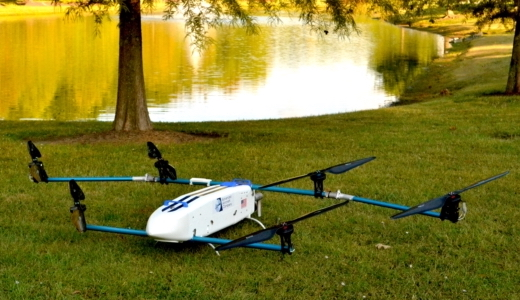
\includegraphics[width=1.0\textwidth]{./img/jpg/uav-HAMR-FuelElectric.jpg}
  \caption{HAMR:~hybrid (fuel+batteries)~\cite{hamrDrone}}%
  \label{fig:uav-hamr-fuel}
\end{subfigure}
  % 
  \begin{subfigure}[t]{0.35\textwidth}
  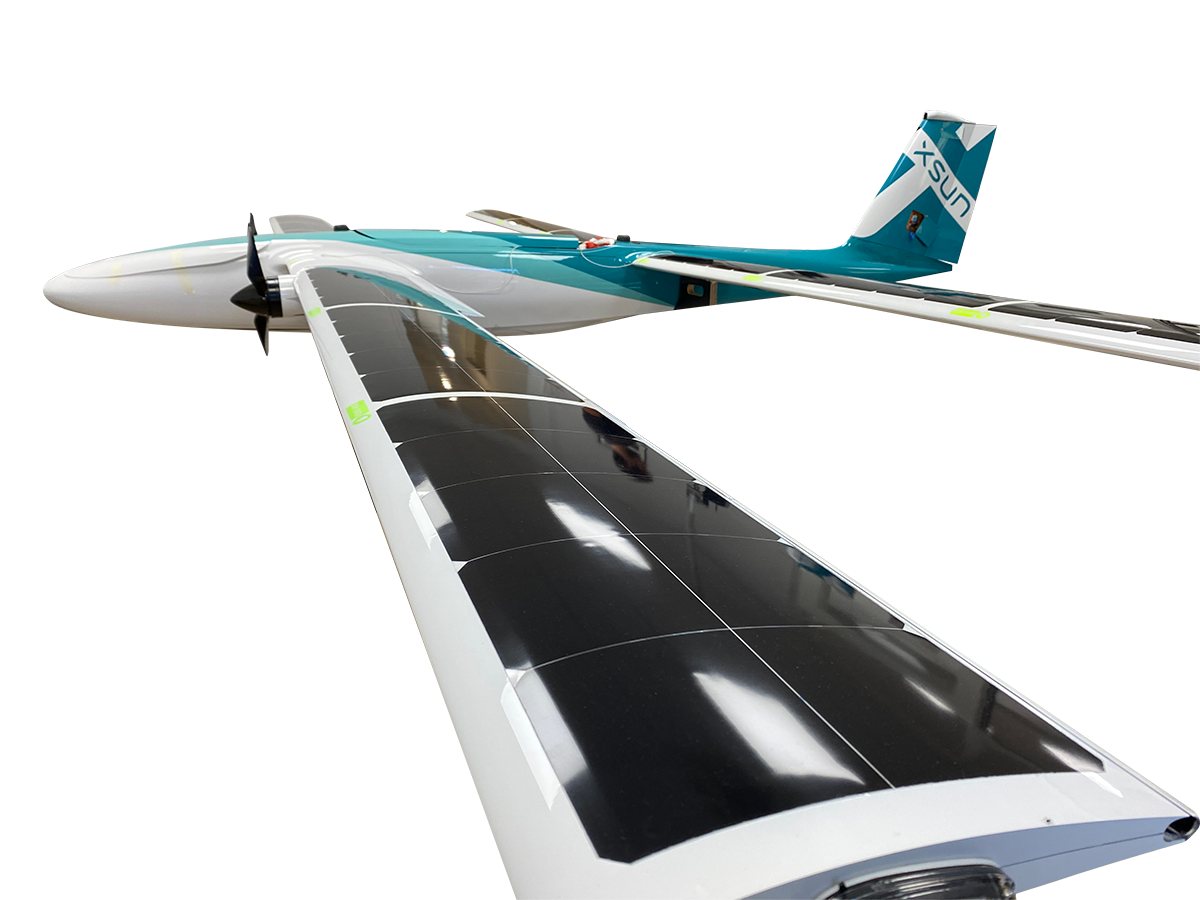
\includegraphics[width=1.0\textwidth]{./img/png/uav-solarXOne.png}
  \caption{Solar X One:~solar powered~\cite{solarXOneDrone}}%
  \label{fig:uav-solarX}
\end{subfigure}
%
  \caption{UAV types}%
  \label{fig:uav-types}
\end{figure}
%

The autonomy or endurance, refers to the maximum flight time with a
single charge (battery, fuel, or both), varying from a 20--30 minutes (small \glspl{uav}) to several
hourse (large \glspl{uav}). Size, weight and weather conditions have a strong
impact on the autonomy. Some technologies are currently being develop to support
in-flight recharging through renewalable sources (\gls{pv} cells) or wireless
power techniques (e.g., laser emission)\cite{mohsan2022towards}.
The payload refers to the lifting capability of the \gls{uav} for load carrying,
varying from few grams (small \glspl{uav}) to hundreds of kilograms (large
\glspl{uav}). Most common payloads are sensors and video cameras~\cite{mohsan2022towards}.
The range defines the distance from where the \gls{uav} can be controlled
remotely and depends on the communication technology and network, and the
weather conditions\cite{mohsan2022towards}. The altitude is the height a drone can fly, weather by
technological constraints or by legal ones~\cite{mohsan2022towards}.
%
Fig.~\ref{fig:uav-mindmap} depicts the \gls{uav}'s
generic overview, summarizing its main concepts.
%
%
\subsection{System overview}%
\label{sec:system-overview}
Fig.~\ref{fig:uav-sysOverv} shows an overview of the \gls{uav} system and its
ecosystem.
Positioned at the center of the figure (1) are the \gls{uav} and its associated flight control \gls{hw} and \gls{sw}.
Its main tasks are path planning, communication
management, data acquisition, and mission~\cite{aggarwal2020UAVPathPlanning}.

\begin{figure}[!hbt]
  \centering
  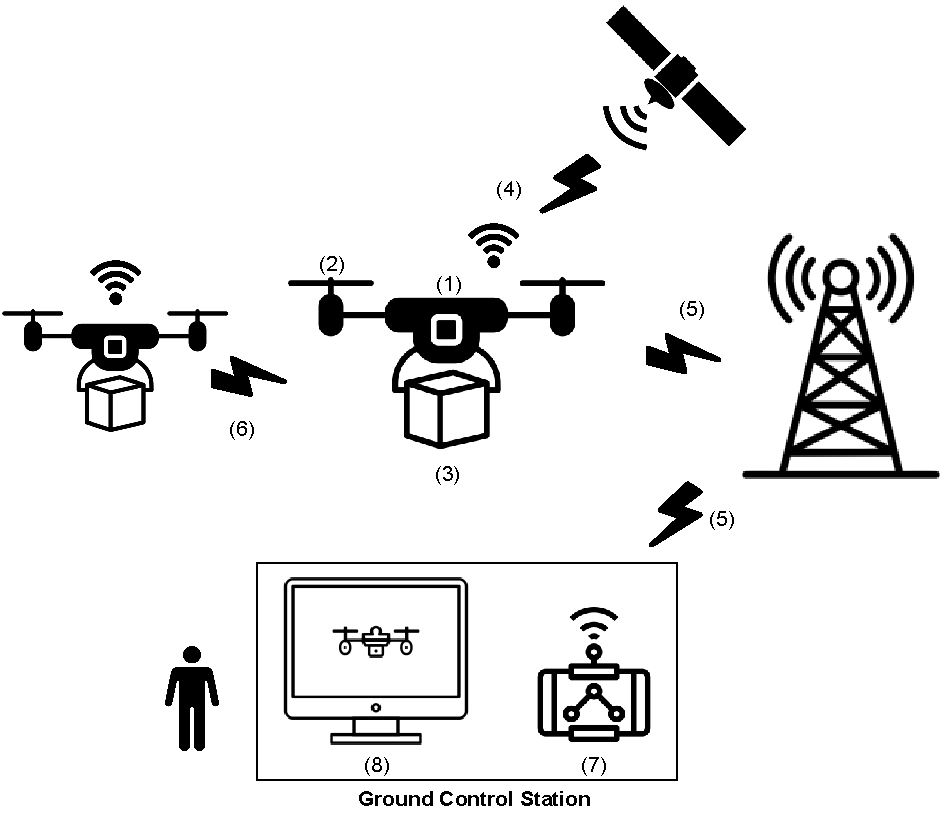
\includegraphics[width=0.7\textwidth]{./img/pdf/uav-sys-overv.pdf} 
%  \includesvg[width=1.0\textwidth]{./img/virtualization.svg} 
  %\caption[Virtualization mind map]{Virtualization mind map}%
  \caption[UAV system overview]{UAV system overview (adapted from~\cite{mohsan2022towards,aggarwal2020UAVPathPlanning})}%
  \label{fig:uav-sysOverv}
\end{figure}

The path planning works in
combination with the \gls{gcs} to assist in the navigation, finding the optimal
path, while providing environmental awareness through weather and climate
monitoring, and controlling the motion and speed for obstacle avoidance. To
achieve this, the
on-board \underline{flight controller} collects data from multiple sensors
(e.g., ultrasonic/infrared sensors for obstacle avoidance,
\gls{imu}, barometer, \gls{gnss}/\gls{gps} module, etc.) and,
together with the commands received from the \gls{gcs}, implements attitude
estimation and the control law (e.g., Kalman filter) to drive the propulsion
system (motors) (2).

The flight controller also manages the communications
between three types of links~\cite{aggarwal2020UAVPathPlanning}: \underline{\gls{uav} to \gls{gcs}} (5) -- radio
communication used for transmitting instrument readings such as audio or video
and for human remote control (7) (8); \underline{\gls{uav}
  to Satellite} (4) -- carries weather, climate, and \gls{gps} information
  required for accurate \gls{uav} navigation; \underline{\gls{uav} to \gls{uav}}
  (6) -- can be used for cooperative missions or to provide environmental
  awareness (e.g., signal danger). The mission refers to the flight's goal,
  e.g., video capturing, topographic mapping, etc., and is directly related to
  the payload (3) (e.g., camera, \gls{lidar}, etc.).

Sensors can be typically categorized into obstacle avoidance, payload, and
navigation~\cite{VogeltanzFreeSWUAVSurvey2016}. Ultrasonic and infrared sensors are generally used to avoid
collisions with obstacle, but \gls{tof} sensors like \gls{lidar} can also be used,
although more expensive and more complex. The navigational sensors include the
\gls{imu} --- used to estimate orientation and heading of the vehicle, the
barometer --- used to estimate of the \gls{uav} with a precision of few
centimeters, and the \gls{gnss}/\gls{gps} module --- used to estimate the
drone's geolocation for navigation and autonomous flight with a precision of up
to 5 meters, thus requiring the \gls{imu} and barometer to improve accuracy~\cite{ebeidUAVPlatformsSurvey2017}.

The actuators depend on the propulsion system, although electronic drives are
always used. For a typical multi-rotor \gls{uav}, \glspl{bldc} motors are used
for rotors, with an \gls{esc} --- an \gls{ac}/\gls{dc} power converter and
high-frequency variable motor speed controller. Fixed-wing hybrids include also
servomotors for flaps~\cite{gabrielBLDCFixedWingUAV2011}.
%
Fig.~\ref{fig:uav-sysOverv-tasks-mindmap} depicts the concept map of \gls{uav}'s
tasks and components.
%
\glspl{uav} can be organized into a top-down hierarchy of layers~\cite{glossner2021overview}, as follows
(see Fig.~\ref{fig:uav-sysOverv-hierarc-mindmap}):
\begin{enumerate}
\item \textbf{Flight Supervision}: the topmost layer handles flight's
  management, safety/authorization, and remote \gls{uav}'s
  identification. \underline{Flight management} is achieved through the
  transmission of commands from the \gls{gcs} to the \gls{uav}'s \gls{fcs}. The \gls{gcs} is
  software running on ground-control devices, and they typically provide path
  planning, mapping and real-time flight statistics superimposed on a map. The
  most notable example is probably \lstinline{QGroundControl}, which provides full
  flight control and setup for \gls{uav} vehicles, cross-platform, and with a
  mobile-styled \gls{ui}. It supports actions to be triggered in case of
  failures (fail-safe features), such as geofencing (limits the permissible fly
  areas). \underline{Safety/authorization} handles the authorization to fly (if
  required) and its safety. Although autopilots, like PX4 and ArduPilot,
  and the \gls{gcs} exist, providing several safety features, the pilot in
  control is ultimately responsible for ensuring the safe flight of any
  \gls{uav}. As such, it must enforce the use of failsafe actions, like in the
  case of low battery, loss of \gls{rc} signal, data link failures, or geofence
  violations, and request authorization to fly if legally demanded. For example,
  pilots can use \lstinline{LAANC} \glspl{api} or
  \lstinline{Google Wing OpenSky} to receive \gls{faa} authorization for entering controlled airspace. On the other
  hand these softwares provides the air traffic professionals drones operations'
  visibility.
  \underline{Remote identification} will be required for all \glspl{uav}
  beginning in 2023. Thus, all \glspl{uav} must be equipped to a \gls{rid}, an
  unique electronic identifier comparable to a vehicle license plate, with direct
  broadcasting of the \gls{rid} to anyone within range of signal.
\item \textbf{Command \& Control}: the second layer ensures drones can fly
  safely, through the transmission of commands to the \gls{uav}, yielded by an
  human operator of computer-generated via autopilot. The command is sent to the
  \gls{uav} via proprietary protocols or open \glspl{api} (e.g., MAVLink
  \gls{sdk} or Parrot \gls{sdk}). The autopilot consists in \gls{sw} stack
  running on the \gls{fcs}. Noticeable open-source autopilots are
  \lstinline{PX4}, \lstinline{ArduPilot}, and \lstinline{Paparazzi}.
\item \textbf{System Simulation}: \gls{uav} behavior is analyzed in respect to
  different environment and conditions, mainly through \underline{flight
    modeling},
  \underline{traffic modelling} --- models real-world traffic interactions
  (land and air) --- and
  \underline{network communication modelling}. 
\item \textbf{Operating Systems}: \glspl{os} are used to interface the
  electronic \gls{hw} that controls \gls{uav} operation through a tractable
  abstraction. \glspl{uav} can a myriad of \glspl{os}, both open-source --- such as
  \gls{ros}, \lstinline{Linux}, \lstinline{FreeRtos}, \lstinline{NuttX}, \lstinline{ChibiOS} --- or proprietary, like \lstinline{VxWorks}. 
\item \textbf{Physical \gls{hw}}: comprises the actual electronic \gls{hw} of
  the \gls{uav}, such as sensors, motors, communications, etc.
\end{enumerate}


\subsection{Security and Safety}%
\label{sec:security-safety}
Another very important feature, often overlooked, is the \gls{uav}'s ecosystem
security, and alongside with it safety of people and goods~\cite{leccadito2018survey}. Security is often
not embedded in the system's design, posing all sorts of problems. For example,
\glspl{uav} often include onboard wireless communication modules that use open,
unencrypted, and unauthenticated channels, exposing them to a variety of
cyber-attacks~\cite{kishnaCyberVulnerUAVReview2017,mansfieldUAVCyberThreats2013}.
The problem is not restricted to
commercial applications, with the U.S. army banning Dji drones --- the most
widely used ones by the army --- for cybersecurity
concerns in 2017~\cite{suasNewsDjiDronesBanned2017}. Hacking of drones is
another major concern, exposing sensitive information and control of the
\gls{uav}. In fact, several incidents have been reported in the media where
drones were weaponized~\cite{spiegelUAVAccident2015,nytimesUAVAccident2018,theDriveUAVAccident2019}, and the volume and risk of such incidents are
likely to increase significantly with the expected drone market growth in the
foreseable future~\cite{mohsan2022towards} and the new regulations adopted by many countries which allow
drones to fly over populated areas~\cite{stocker2017UAVRegulationsReview}.

The most common attacks to the  \gls{uav} are \gls{dos} and \gls{ddos}, causing
resource availability challenges which can be exploited to drain the batteries,
overload the processing units, and flood the communications link, leading to
huge services' interruption~\cite{mohsan2022towards}. But more sophisticated attacks are used too, like
\gls{gps} spoofing --- impersonating as a valid \gls{gps} satellite to provide
false data, \gls{gps} jamming, instrument spoofing (gyroscope, compass), or even
killing the main process~\cite{nassi2021sok}. Ground control stations are a target too, since the
attacker can indirectly obtain access to the \gls{uav}, usually through key
loggers, viruses, and malwares,  and steal all of its data or send malicious
and erroneous commands to the \gls{uav}~\cite{mohsan2022towards}.

Nassi et al.~\cite{nassi2021sok} conducted a thorough and very extensive survey
on the security and privacy issues associated with \glspl{uav}, the attacks and countermeasures. The authors
divided the security attacks on two categories:
\begin{itemize}
\item \textbf{Targetting \glspl{uav}}: corresponds to an attack an
  ill-intentioned civilian performs on an \gls{uav} using, e.g., an \gls{sdr}, a
  computer or a commercial laser. Six targets were identified --- the \gls{uav}
  electronic \gls{hw}, the \gls{uav} chassis and package (e.g., propelers and
  cargo), the \gls{gcs}, the \gls{fpv} channel, the pilot and cloud
  services/servers. Attacks on the \gls{uav} \gls{hw} include installation of
  fake firmware, instrument spoofing and \gls{gps} jamming. Countermeasures vary
  with each attack, but, for example, the installation of fake firmware on the
  device can be opposed by requiring the digital signature of the firmware
  before installing. Direct attacks to interrupt \gls{uav}'s flight control and
  commiunications links to modify mission parameters can be mitigated through
  onboard \gls{sw} and \gls{hw} mechanisms, such as real-time monitoring,
  instantaneous estimation of the controller, alert warning and immediate action
  on any alteration from the intended controller model~\cite{mohsan2022towards}.
  Attacks on the chassis and package include fake \gls{cad}
  files to undermine its fabrication and deployment, especially critical for
  open-source \gls{hw}, nets, and bullets. They can be opposed by requiring
  digital signature and by using parachutes, respectively.
  The \gls{fpv} channel is the radio communication channel between the \gls{uav}
  and the \gls{gcs}, which enables the pilot to fly as if it was on board and
  consists of a downlink --- used for video streaming --- and an uplink --- used
  to control the \gls{uav} via the \gls{gcs}. The most known methods are
  pilot's deauthentication, taking and dowloading videos and pictures, killing
  the main process, or remote control of the drone, which can be mitigated
  through the usage of an encrypted network protocol. Jamming is also an issue
  and can be remediated using channel hopping. Lastly, cloud services and
  servers expose the \gls{uav} indirectly to hackers, because, although most
  \glspl{uav} are not connected to the Internet, the \gls{gcs} is, sending the
  telemetry of flights to cloud servers for storage and analysis. The methods
  used to explore this link are deanonymizing pilots and extracting flight
  history, which can be both mitigated through the implementation of
  authorization and two-factor authentication mechanisms.
\item \textbf{Targetting people}: \glspl{uav} can attack people, on a
  individual, organization or nation base. The countermeasures include
  \underline{detection and tracking}, \underline{assessment}, and
  \underline{interdiction}. Several detection methods exist, such as radars,
  video and infrared cameras, \gls{lidar}, acoustics, acoustics and optics,
  etc. However, it is important to note that none of these methods are
  fail-proof. For example, specific radars have to be used with very specialized
  operators, since common radars are designed for large aircraft detection and
  drones uses materials which are not very radio reflective. Another example is
  the acoustics, where sensors exist to detect the specific spectrum of the
  drone's propellers, but can be easily circumvented by going into silent
  (stealth) mode~\cite{sathyamoorthy2015review}. Assessment concerns the rating
  and identification of hostile drones, especially important in areas where
  drones are used for both legal and illegal activies. The most used methods are
  based on \gls{uav}'s classication, to identify the manufacturer and model of
  the drone. In the event of the detection and assessment of a hostile drone,
  interdiction must be applied, i.e., the drone should be disabled. For this
  purpose, several methods can be used like bullets and nets, which are
  dangerous and not very effective, commercial jammers, predator birds and laser
  cannons.
\end{itemize}

Safety failures are also very serious, since they pose risks on the integrity of
people and goods. They can be categorized as follows~\cite{ferrao2020stuart}:
\begin{itemize}
\item \textbf{Damague due to calculation errors}: occurs when a \gls{uav} is
  more dangerous than planned. For example, in 2020 in the U.K., an activist
  group piloted hundreds of drones with the 3-mile depletion zone to interrupt
  the flights, which could have been catastrophic.
\item \textbf{Sensor failures}: \gls{uav} sensors do not easily detect delicate
  objects, such as wires, tree branches, and transparent surface such as
  buildings windows. Falls by collisions with these types of objects are very
  common due to undetected obstacle or pilot's excess of confidence.
\item \textbf{Obstacle deviation}: collisions and crashes caused by object
  deviation are common, from building to trees.
\item \textbf{Direct attacks}: these attacks are performed to harm people, for
  personal or ideological reasons, or to steal the \gls{uav} payload, e.g., an
  organ, food, or vaccines. The recreational/hobbyist \glspl{uav} are the most
  commonly targets.
\item \textbf{Accidental damage}: can occur when a \gls{uav} gets out of
  control, due to legitimate loss of control by the owner, cyber attack, or
  \gls{sw} or \gls{hw} malfunction. Indepently of the cause, the extent of the
  damage on people as goods can be severe, due to crash of \gls{uav} falling
  from the sky.
\end{itemize}

Clearly, security and safety are fundamental aspects of the \gls{uav}'s
operation, but they require more effort to decrease the attack vectors and the
attack surface. Ferrão proposed that \gls{uav}'s design considers simultaneously
both aspects, as they strongly influence each
other~\cite{ferrao2020stuart}. Fig.~\ref{fig:uav-security-mindmap} illustrates the
\gls{uav}'s security and safety taxonomy.

\subsection{UAV Reference Hardware}%
\label{sec:uav-ref-hw}
In this section we discuss the reference hardware for \glspl{uav}.
Firstly, we present an overview over the \gls{hw} architecture. Then, we analyze
in more depth the open-source and commercial hardware solutions for \glspl{uav}.

\subsubsection{Overview and Architecture}%
\label{sec:overv-arch-hw}
Fig.~\ref{fig:uav-hw-arch} illustrates the high-level abstraction of the
\gls{uav} \gls{hw} architecture~\cite{leccadito2018survey,px4-sysArch}. The main
computing platforms are depicted in orange: (1) the flight controller or
\gls{fmu} (e.g., Pixhawk); (2) and, optionally,
the companion computer, which provides extra functionalities, off-loading the \gls{fcs}. More specifically, the companion computer can assist in the
navigation, preventing collisions and avoiding obstacles, support
mission-related tasks like camera surveillance or topographic mapping, and
process telemetry data.

\begin{figure}[!hbt]
  \centering
  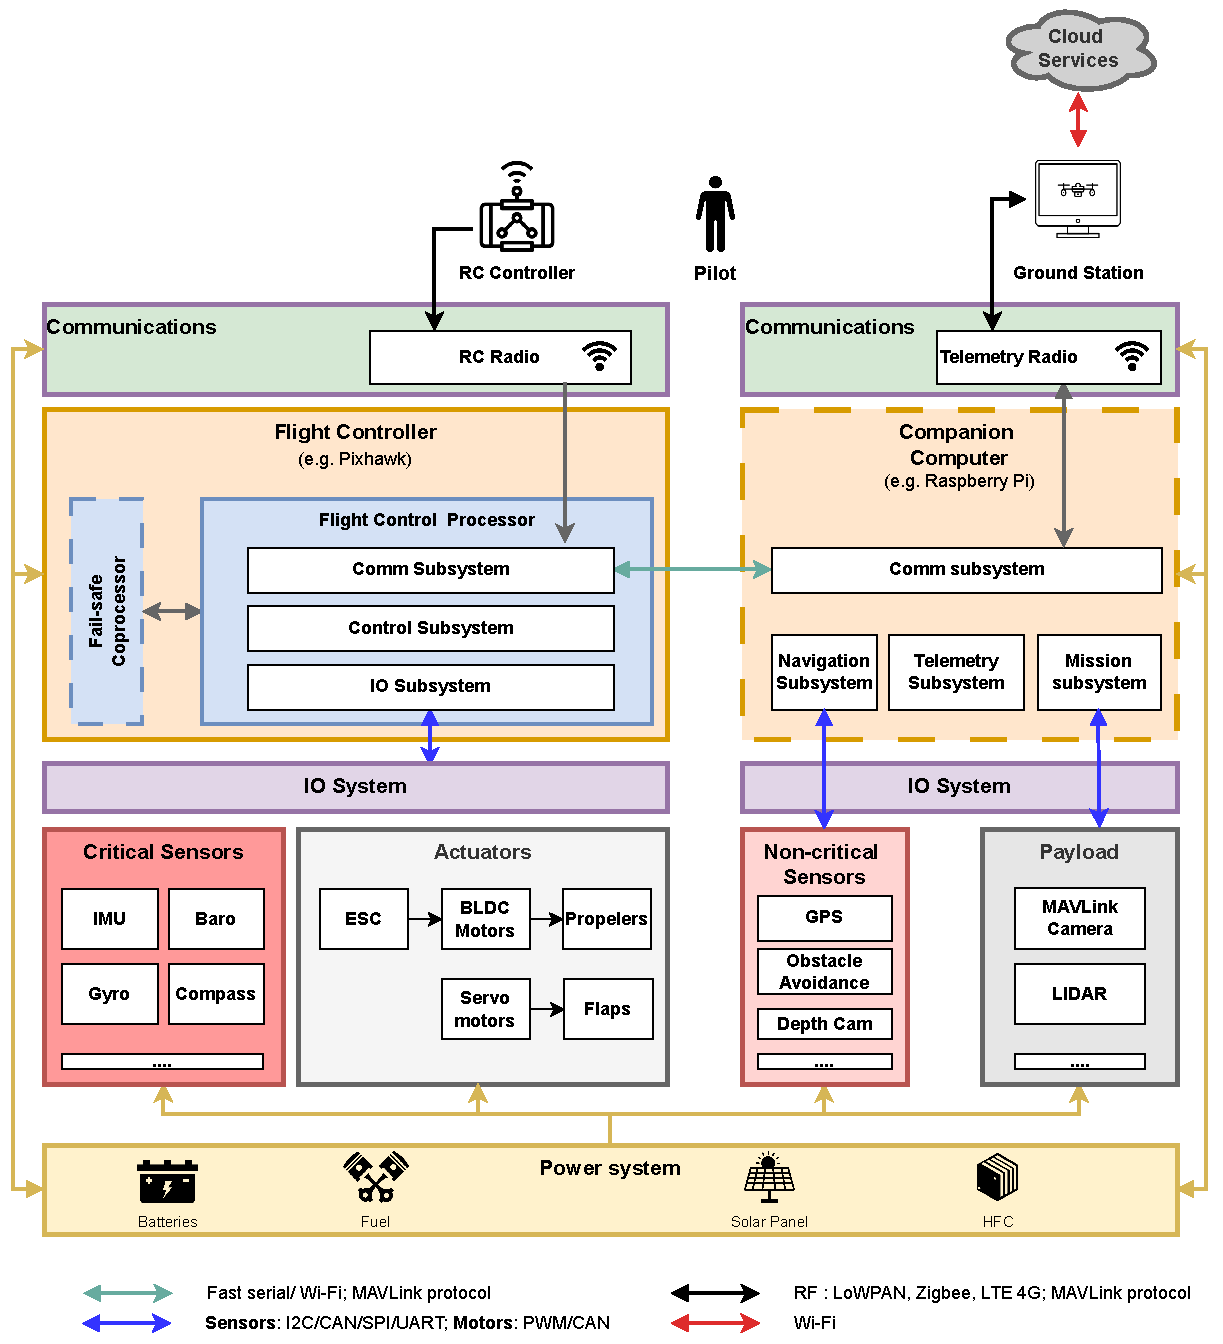
\includegraphics[width=1.0\textwidth]{./img/pdf/uav-hw-arch.pdf} 
  %\caption[Virtualization mind map]{Virtualization mind map}%
  \caption{UAV HW architecture: high-level abstraction}%
  \label{fig:uav-hw-arch}
\end{figure}

The \gls{fcs} is typically composed of a main processor, for \gls{uav} control,
and a optionally fail-safe coprocessor, dedicated to respond to failure events,
e.g., returning to base when the battery reaches the low threshold.
The main processor handles: (1) communications: processing commands arriving
from the manual \gls{rc} controller or between the companion computer; (2)
aircraft's control: typically using \gls{pid} models and/or estimation methods
(e.g., Kalman filter): (3) \gls{io}: to
interface the critical sensors, such as \gls{imu}, barometer, gyroscope, and
compass, or the actuators, such as \gls{bldc} motors and servomotors.
The power system supplies the required energy for computing and \gls{io}.

As aforementioned, the flight controller does not explicitly require the
companion computer, since the commands sent manually by the pilot
through the \gls{rc} controller are sufficient to control the aircraft flight
(\gls{los} navigation). However, for autonomous missions, the non-critical
sensors such as the \gls{gps} and obstacle avoidance sensors are mandatory. In
this mode, the companion computer sends telemetry data to the \gls{gcs}, which
are typically superimposed on a map for straightforward navigation and receives
the navigational and mission-related commands, processing them and dispatching
the lower level commands to the flight controller or \gls{io} system.

\subsubsection{Open-source solutions}%
\label{sec:open-source-solut-hw}
\glsxtrfull{osh} solutions have been developed to provide more transparency,
extensibility, flexibility, maintainability, while trying to be
cost-effective. \gls{osh} means that the \gls{hw} design (i.e., mechanical
drawings, schematics, \gls{bom},\gls{pcb} layout data, \gls{hdl} source code),
and the \gls{sw} that drives the \gls{hw}, are all released under free/libre
terms~\cite{freeGNU}.
The user can purchase or manufacture the \gls{hw} components
individually or in \gls{cots} kits.

The \gls{osh} solutions fall into three main categories: Atmel-based,
ARM-based, and Companion Computer-based
platforms~\cite{ebeidUAVPlatformsSurvey2017}. The first two target the
\gls{fmu}, while the last provides a \gls{fmu} + companion-computer solution in
one package. Until recently, the Atmel-based platforms, such as the HobbyKing
KK.2.1.5, were still being produced. This product featured an Atmel Mega644PA
8-bit AVR with 64 KB of memory, a MPU-6050 \gls{imu} sensor, and a \gls{lcd} and
push buttons for user interaction~\cite{hobbykingKK2}. It came pre-installed
with the KK2 firmware, but it could also run the ArduPilot software
stack. Another notable example was the ArduPilot Mega (APM), based on the
8-bit ATmega 2560 \gls{mcu}, which includes an \gls{imu} and, optionally, q
compass and a \gls{gps}~\cite{ardupilotMega}. Its biggest advantage is that it could be programmed using the
Arduino \gls{ide}, enabling easy customization of the ArduPilot firmware's
features by hobbyists. The complexity level of modern autopilots require more
powerful \gls{mcu}, dictating the deprecation of the 8-bit ones~\cite{fmu8BitDeprecation}.  

Currently, the vast majority of \gls{osh} projects are based on 32-bit ARM platforms
(\lstinline{Pixhawk 4}, \lstinline{CC3D}, \lstinline{Paparazzi Chimera},
\lstinline{CUAV v5 Plus}, etc.) and supported by initiatives
like the Pixhawk \gls{hw} standardization. Pixhawk is a company that develops open
standards for drone hardware, providing readily available \gls{hw}
mechanical and electrical specifications and guidelines for drone development~\cite{pixhawk}.
%
The \lstinline{Pixhawk 4} (see Fig.~\ref{fig:osh-pixhawk4}) is a flight
controller developed in collaboration by the Holybro manufacturer and the PX4
\gls{sw} teams, and suitable for academic and commercial developers~\cite{pixhawk4}.
It was released under the \gls{bsd} license, comprising two 32-bit ARM
processors: an Cortex-M7 STM32F765 as the main \gls{fmu} processor and a
Cortex-M3 STM32F100 as an \gls{io} coprocessor. The Pixhawk 4 comes with
on-board sensors (accelerometers/gyroscopes, magnetometer, and barometer) and a
\gls{gps} module, and supports the \gls{pwm}, \gls{can} \gls{i2c}, \gls{uart},
\gls{spi}, for sensors and actuators operation. The \gls{uart} and telemetry
interfaces are also available for communication with an off-board
computer~\cite{pixhawk4} and remote controller. The Pixhawk 4 runs the PX4
autopilot on top of the NuttX \gls{rtos}.
%
The \lstinline{CUAV v5 Plus} is another flight controller that uses the dual Arm
Cortex-M7 architecture for \gls{fmu} and \gls{io}~\cite{arduPilot-cuavV5}. It
was released under the \gls{bsd} license and runs the ArduPilot
firmware. On the other hand, the \lstinline{Paparazzi Chimera} is an \gls{osh}
flight controller that integrates all \gls{io} in the same same board, based on
a ARM Cortex-M7 STM32F767 \gls{mcu}~\cite{paparazziChimera}. It was released
under the \gls{gpl} license and runs the Paparazzi
autopilot~\cite{paparazzi-github}. All the ARM-based platforms feature small
on-board memory, typically up to 2 MB of Flash memory and 512 KB of \gls{sram} memory.
  
% Pixhawk 4
\begin{figure}[!hbt]
  \centering
  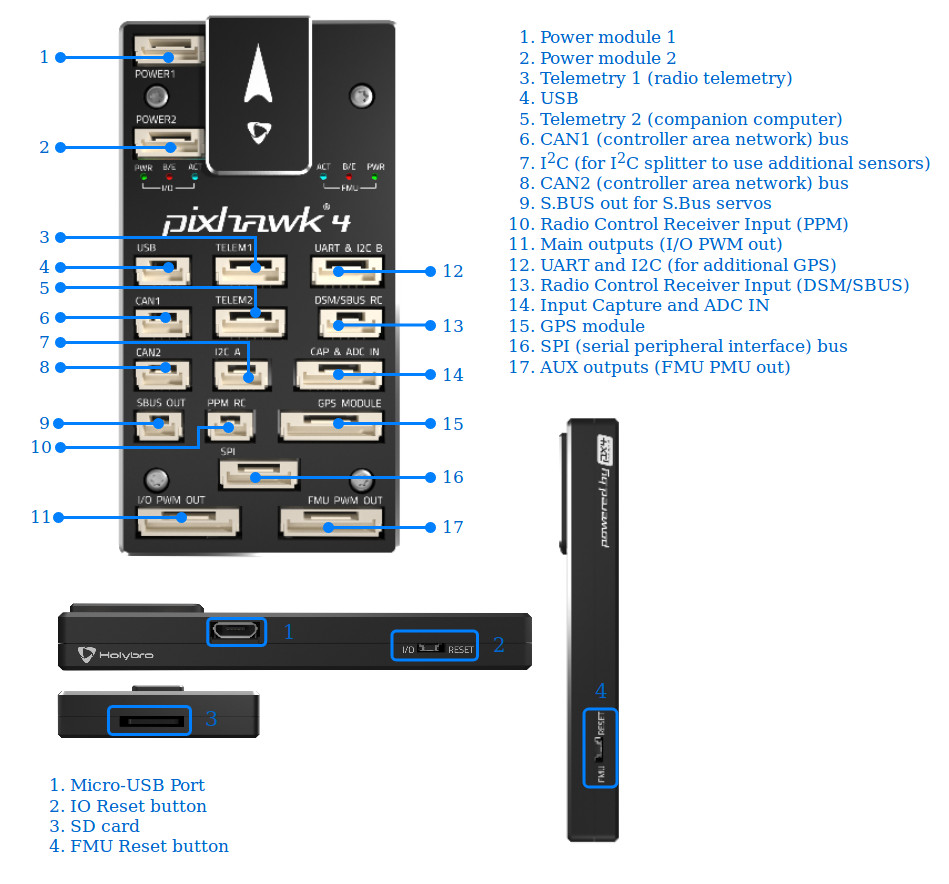
\includegraphics[width=0.7\textwidth]{./img/jpg/osh-pixhawk4.jpg} 
  \caption[Pixhawk4 flight controller]{Pixhawk 4 flight controller~\cite{pixhawk4}\footnotemark}%
  \label{fig:osh-pixhawk4}
\end{figure}
\fnlicCCFour{foot:cc-lic}% CC licence

The companion computer-based platforms expands \gls{io} functionality through a daughter
board, like the Erle-Brain 3 or PXFmini~\cite{ebeidUAVPlatformsSurvey2017}, while using the Arm Cortex-A to run a
custom Linux \gls{gpos} with a preemptive kernel option that hosts the flight
control stack~\cite{erle-brain}. The PXFMini, for example, weighs only fifteen
grams and was assembled on top of a single-core Raspberry Pi Zero, providing
on-board barometer and \gls{imu} sensors, expansion ports, and a triple
redundant power supply~\cite{pxfmini}. Unfortunately, the Erle-Brain 3 and PXFmini were
deprecated after the Erle Robotics company was bought out~\cite{pxfmini-deprec}.
%
The PilotPi shield is another RaspberryPi-based platform, but targetted for hobbyists. The PilotPi shield provides a fully functional open-source
solution for running PX4 autopilot directly on Raspberry Pi, requiring no
proprietary drivers while offering open-source \gls{pcb} and
schematics~\cite{px4-pilotpi}.


  % This flight controller integrates all \gls{io} in the same board, and it uses the  @ 216 MHz (2 MB Flash,
  % 512 Kb \gls{sram}) \gls{mcu}. It comes with on-board sensors
  % (\gls{imu}, barometer, and pressure sensure), an XBEE modem holder for
  % communications, and a dedicated serial link and power supply for the companion
  % computer (e.g., Beaglebone, RaspberryPi, etc.).

%   It has \gls{pwm}, \gls{can}
%   \gls{i2c}, \gls{uart}, \gls{spi}, and servomotors interfaces~\cite{pixhawk4}.
  
% % Paparazzi Chimera
% \begin{figure}[!hbt]
%   \centering
%   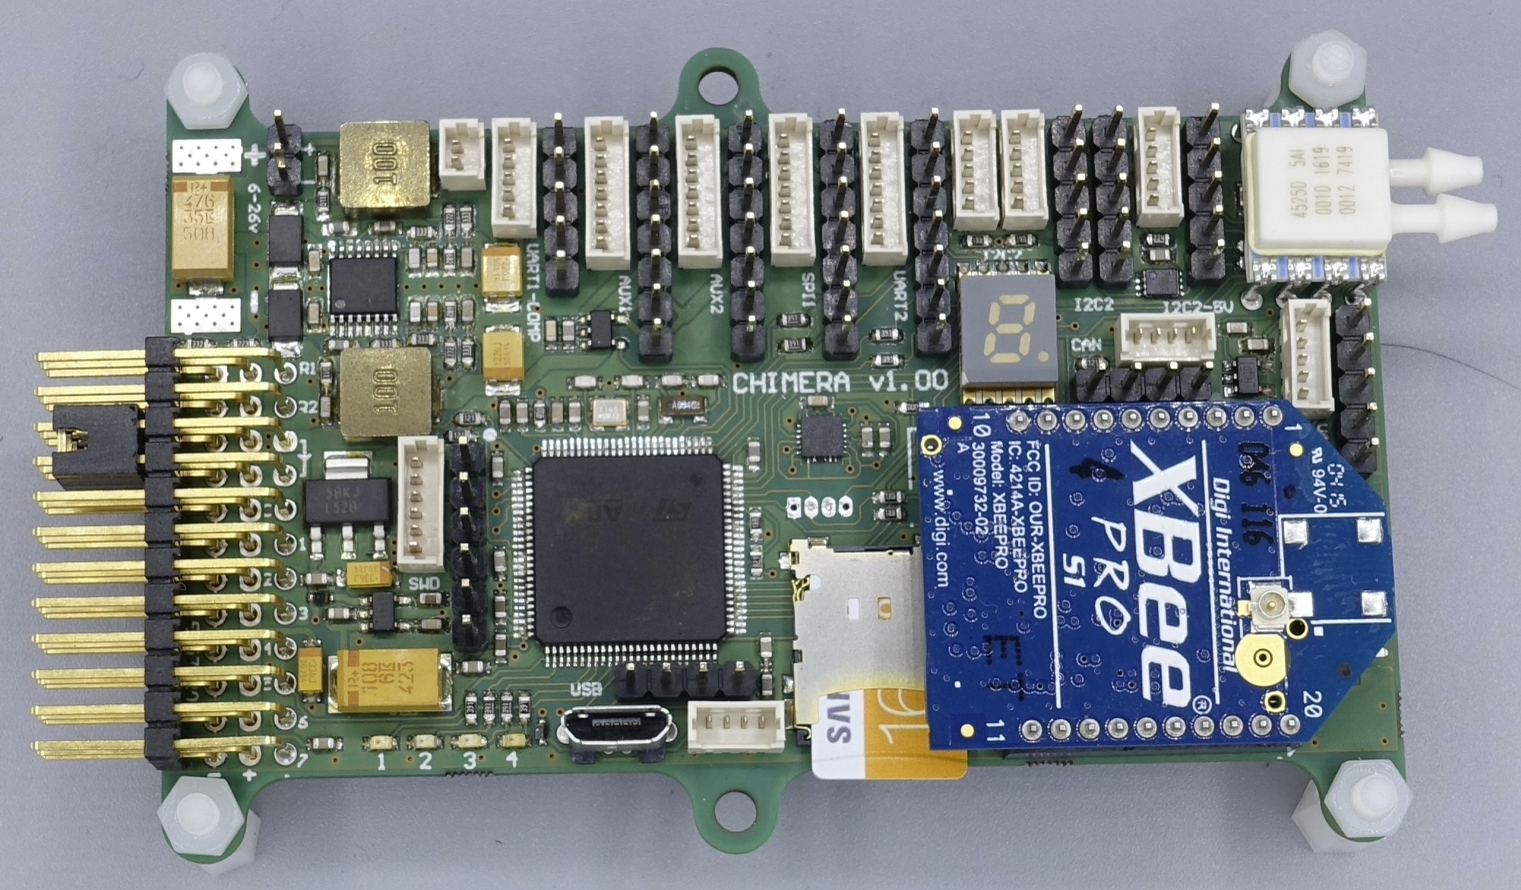
\includegraphics[width=0.6\textwidth]{./img/png/osh-paparazzi-chimera.png} 
%   \caption{Paparazzi Chimera flight controller~\cite{paparazziChimera}}%
%   \label{fig:osh-paparazzi-chimera}
% \end{figure}
  
%   The \lstinline{CC3D} is an \gls{osh} flight controller released
%   under the \gls{gpl} license~\cite{cc3d} (see
%   Fig.~\ref{fig:osh-cc3d}), running the \lstinline{OpenPilot} firmware. It uses a STM 32-bit \gls{mcu} @ 90
%   MHz (128 kB Flash and 20 kB \gls{sram}). It comes with on-board gyroscope and
%   accelerometers, support to serial and \gls{usb} telemetry, up to ten motors,
%   and provides camera stabilization.
  
% % CC3D
% \begin{figure}[htb!]
%   \centering
%   %
%   \begin{subfigure}[t]{0.8\textwidth}
%   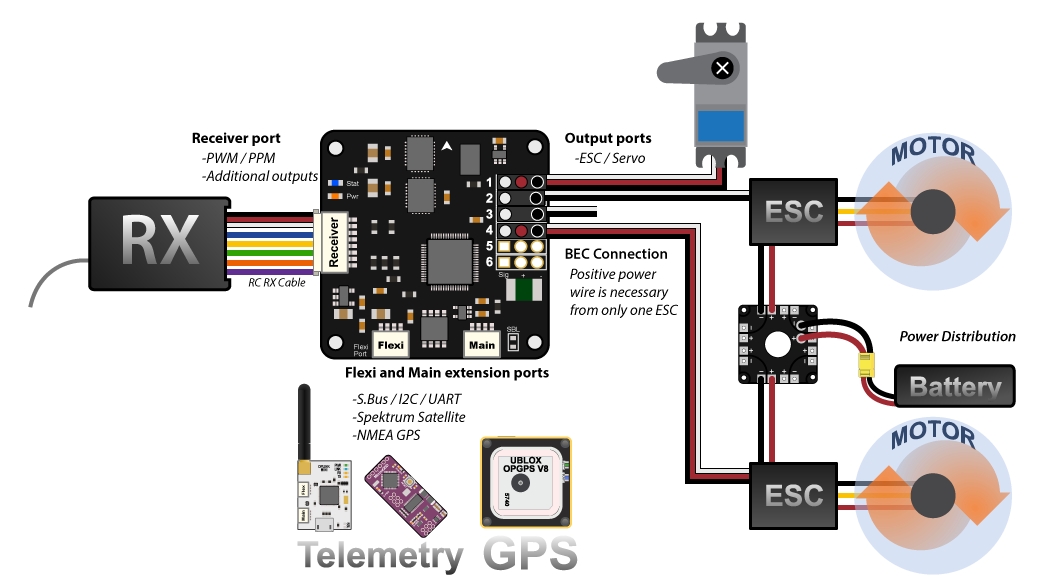
\includegraphics[width=1.0\textwidth]{./img/png/osh-cc3d-conn.png}
%   \caption{Connection diagram}%
%   \label{fig:osh-cc3d-conn}
%   \end{subfigure}
% %
%   \begin{subfigure}[t]{0.35\textwidth}
%   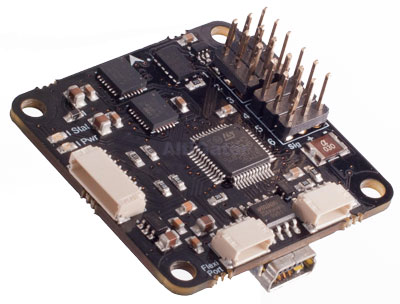
\includegraphics[width=1.0\textwidth]{./img/png/osh-cc3d-board.png}
%   \caption{flight controller board}%
%   \label{fig:osh-cc3d-board}
% \end{subfigure}
% %
%   \caption{CC3D flight controller~\cite{cc3d}}%
%   \label{fig:osh-cc3d}
% \end{figure}
% %
  
% CUAV V5 Plus
% \begin{figure}[!hbt]
%   \centering
%   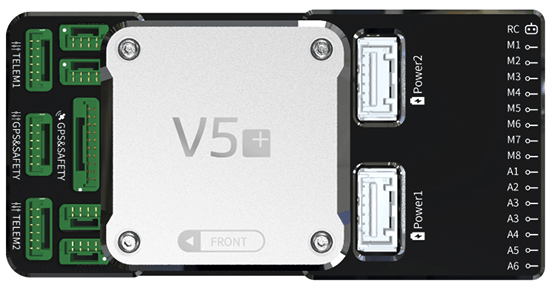
\includegraphics[width=0.6\textwidth]{./img/png/osh-cuav-v5.png} 
%   \caption{CUAV v5 Plus flight controller~\cite{arduPilot-cuavV5}}%
%   \label{fig:osh-cuav-v5}
% \end{figure}

\subsubsection{Commercial solutions}%
\label{sec:commercial-solutions-hw}
The commercial solutions are generally proprietary in nature, and thus closed-source. The
lack of transparency can be an issue, raising suspicions, like the on-going ban
of the U.S. Army to the Dji
drones~\cite{suasNewsDjiDronesBanned2017,djiBan2022}. Nonetheless, proprietary
solutions represent 70\% of the market share, with Dji being the biggest
manufacturer~\cite{droneAnalyst2021}.
%
The commercial solutions can be classified into three main categories: microcontroller-based, \gls{fpga}-based, and Companion Computer-based
platforms.
The \lstinline{SPRacing H7 Extreme} is a low-end flight controller featuring the
Arm STM32H750 \gls{mcu}~\cite{spRacing}
with an external 128 MB flash
memory and all the common onboard sensors and interfaces. Targetted for the \gls{uav} racing market, it supports \gls{fpv} video
streaming through the available camera interfaces~\cite{spRacing}. The
Betaflight or Cleanflight \gls{sw} stack is commonly used in the racing
\glspl{uav} such as this one, although it is compatible also with the \lstinline{ArduPilot} stack~\cite{arduPilot-SPRacing}.

% \paragraph{Microcontroller-based platforms}
%  

% SPRacing H7 extreme
% \begin{figure}[htb!]
%   \centering
%   %
%   \begin{subfigure}[t]{0.25\textwidth}
%   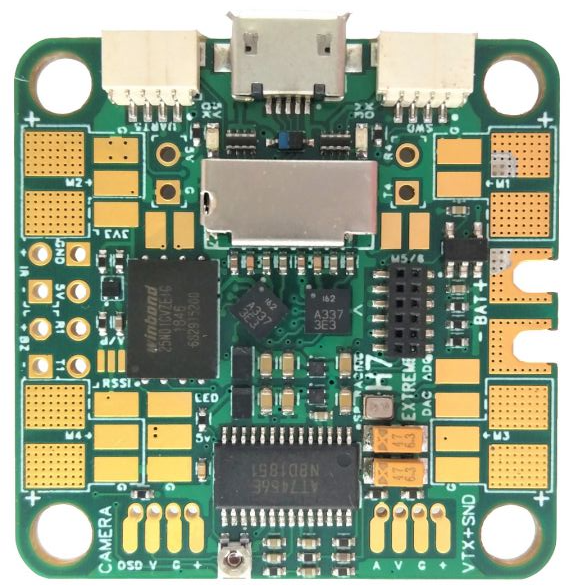
\includegraphics[width=1.0\textwidth]{./img/png/hw-SPracing-H7-extreme.png} 
% %  \caption{Connection diagram}%
% %  \label{fig:osh-cc3d-conn}
%   \end{subfigure}
% %
%   \begin{subfigure}[t]{0.25\textwidth}
%   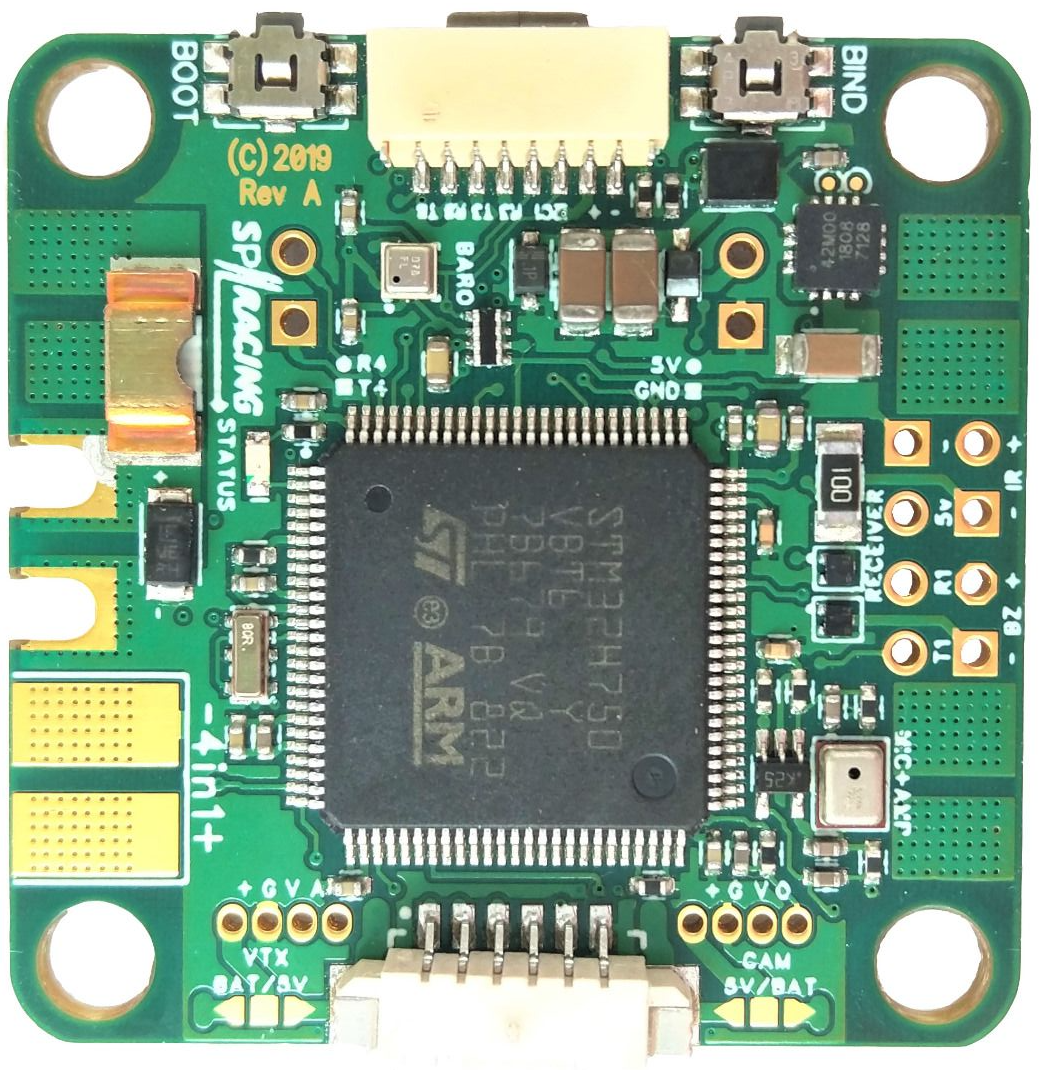
\includegraphics[width=1.0\textwidth]{./img/png/hw-SPracing-H7-extreme2.png} 
%  % \caption{flight controller board}%
%  % \label{fig:osh-cc3d-board}
% \end{subfigure}
% %
%   \caption{SPRacing H7 extreme flight controller~\cite{arduPilot-SPRacing}}%
%   \label{fig:hw-SPRacing}
% \end{figure}
%

% \paragraph{FPGA-based platforms}
The \lstinline{Aerotenna OcPoC-Zynq Mini} is a \gls{fpga} + ARM \gls{soc} based
  flight control platform,  which supports the ArduPilot and PX4 \gls{sw}
  stacks~\cite{ocpoc} (see Fig.~\ref{fig:hw-ocpoc}). Released back in 2017, it
  is currently discontinued~\cite{ocpoc-discontinued}.
  The Artix-7 \gls{fpga}, with 28 thousand logic cells, provided \gls{ai}
  capabilities and \gls{io}'s flexibility, crucial for rapid sensor integration
  and customization of the flight controller \gls{hw}. The ARM Cortex-A9
  dual-core runs Linux for data logging and processing, and includes 512 MB
  \gls{ram} and 128 MB of flash memory. The OcPoc-Zynq Mini supported
  triple-redundancy in the \gls{gps}, magnetometers, and \glspl{imu} on top of
  the conventional on-board sensors, programmable in the
  \gls{fpga}~\cite{ocpoc}.

% Ocpoc
\begin{figure}[!hbt]
  \centering
  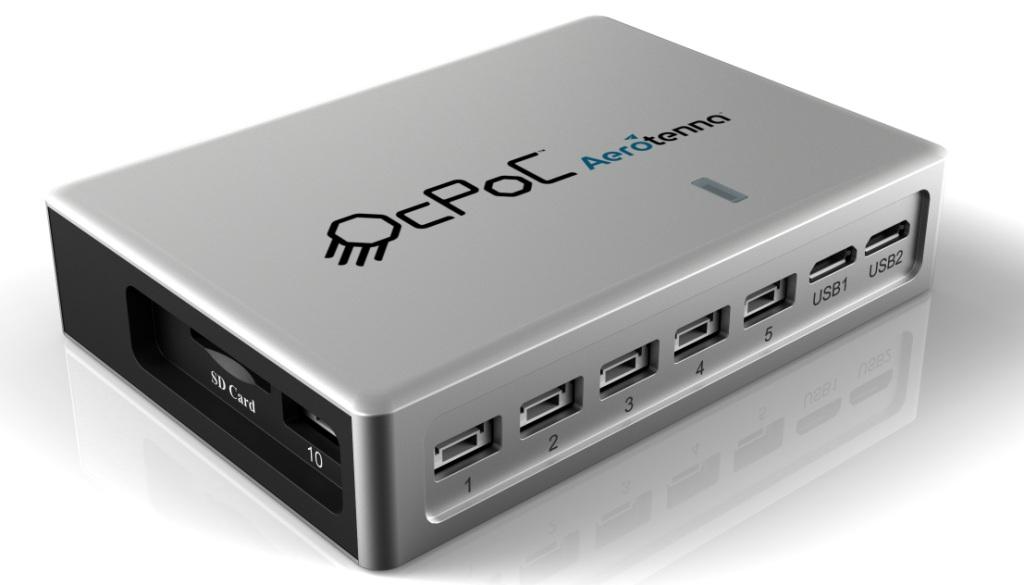
\includegraphics[width=0.5\textwidth]{./img/png/hw-ocpoc-zynq-mini.png} 
  \caption[Aerotenna OcPoc-Zynq Mini flight controller]{Aerotenna OcPoc-Zynq Mini flight controller~\cite{ocpoc}\footnotemark}%
  \label{fig:hw-ocpoc}
\end{figure}
%
\fnlicCCFour{foot:ocpoc}%

%\paragraph{Companion Computer-based platforms}
The most notable companion computer-based platforms are the Navio2,
the PixC4-Jetson, and the Auterion Skynode X/S.  
Similarly to PilotPi, the \lstinline{Navio2} flight controller consists of a
Raspberry Pi shield, but the hardware design is closed-source.
Navio2 runs a custom version of the Raspberry Pi OS (debian-based)~\cite{navio2-sw}, which supports ArduPilot and PX4 \gls{sw}
stacks~\cite{arduPilot-Navio2,navio2-px4}.
  The shield includes on-board
  sensors (dual \gls{imu}, barometer), a \gls{gnss} receiver, an \gls{rc}
  \gls{io} coprocessor, \gls{i2c}, and
  \gls{uart} interfaces for sensors and radios, 14 \gls{pwm} servomotors
  outputs, and a triple redundant power supply~\cite{arduPilot-Navio2}.

% NAVIO2
% \begin{figure}[!hbt]
%   \centering
%   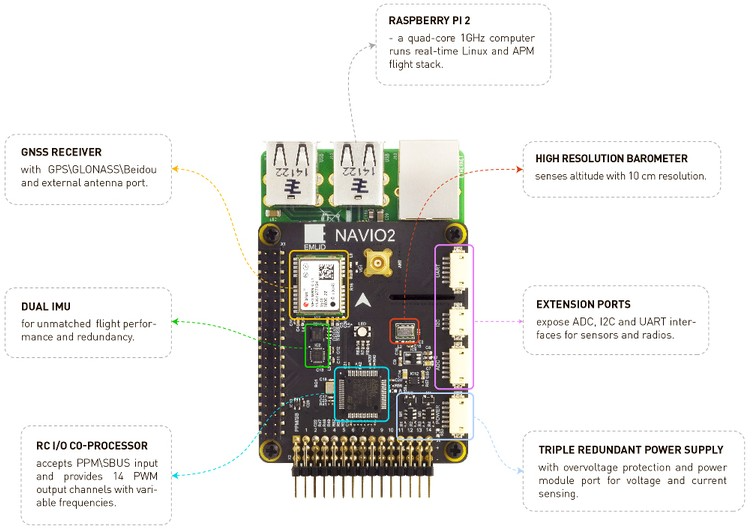
\includegraphics[width=1.0\textwidth]{./img/png/osh-NAVIO2} 
%   \caption{NAVIO2 flight controller~\cite{arduPilot-Navio2}}%
%   \label{fig:osh-NAVIO2}
% \end{figure}

  The \lstinline{PixC4-Jetson} (Fig.~\ref{fig:hw-horizonJetson}) is a
  professional high-end flight controller that integrates an dual-ARM
  \gls{fmu} and \gls{io} processors, and the Nvidia Jetson companion
  computer~\cite{arduPilot-horizonJetson}. This flight controller supports the
  ArduPilot and PX4 \gls{sw} stacks and can be remotely configured through a
  remote terminal~\cite{arduPilot-horizonJetson}. Thus, extra security measures are required, with the
  PixC4-Jetson providing a \gls{lte} connection management with a Layer-2 peer
  to peer \gls{vpn} and a secure cloud connection to Horizon31's
  U.S. servers~\cite{arduPilot-horizonJetson}. The live video streaming is
  assured by multiple-endpoint encoding pipelines and optional access to
  Horizon's cloud low-latency web\gls{rtc} video distribution system.
  %
  The Nvidia Jetson companion computer is well-suited fo computer vision,
  machine learning, and \gls{ai} tasks, further enhancing the capabilities of
  the \gls{uav}~\cite{jetson-docs}.

% Horizon Jetson
\begin{figure}[htb!]
  \centering
  %
  \begin{subfigure}[t]{0.9\textwidth}
  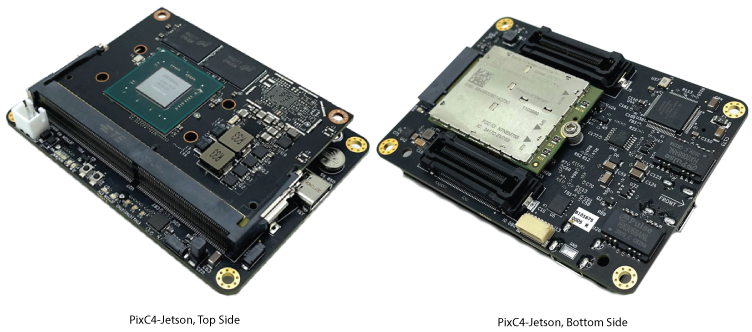
\includegraphics[width=1.0\textwidth]{./img/png/hw-horizon-pixc4-jetson.png} 
  \caption{Board}%
  \label{fig:hw-horizonJetson-board}
  \end{subfigure}
%
  \begin{subfigure}[t]{0.9\textwidth}
  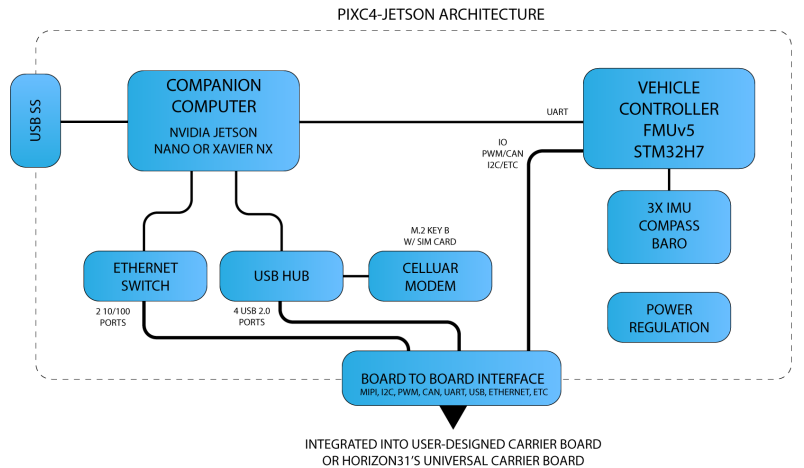
\includegraphics[width=1.0\textwidth]{./img/png/hw-horizon-pixc4-jetson-arch.png} 
  \caption{HW architecture}%
  \label{fig:hw-horizonJetson-arch}
\end{subfigure}
%
  \caption[Horizon31 PixC4-Jetson flight controller]{Horizon31 PixC4-Jetson flight controller~\cite{arduPilot-horizonJetson}\footnotemark}%
  \label{fig:hw-horizonJetson}
\end{figure}
%
\fnlicCCFour{foot:jetson-hw-sw}%

% Skynode X
Another relevant option in the commercial market is the \lstinline{Auterion Skynode X},
combining a flight controller, a mission computer and \gls{lte} connectivity all
in on product~\cite{skynodeXWebsite} in a compact form factor.
%
The \gls{fmu}, based on the Pixhawk FMUv6 architecture, comprises the 
a STM32H753 microcontroller and the STM32F103 \gls{io} coprocessor, and a
triple-redundant inertial sensor to minimize failure risk~\cite{skynodeXDatasheet}.
It supports up to 8 \gls{uart}, a dual redundant \gls{can},
100Base-TX Ethernet, 16 \gls{pwm} outputs, 2 \gls{i2c} and 1 \gls{spi}
connections. The \gls{fmu} runs an enterprise-hardened version of PX4, labelled
as Auterion PX4 (APX4)\cite{skynodeXDatasheet}.
%
% \begin{figure}[!hbt]
%   \centering
%   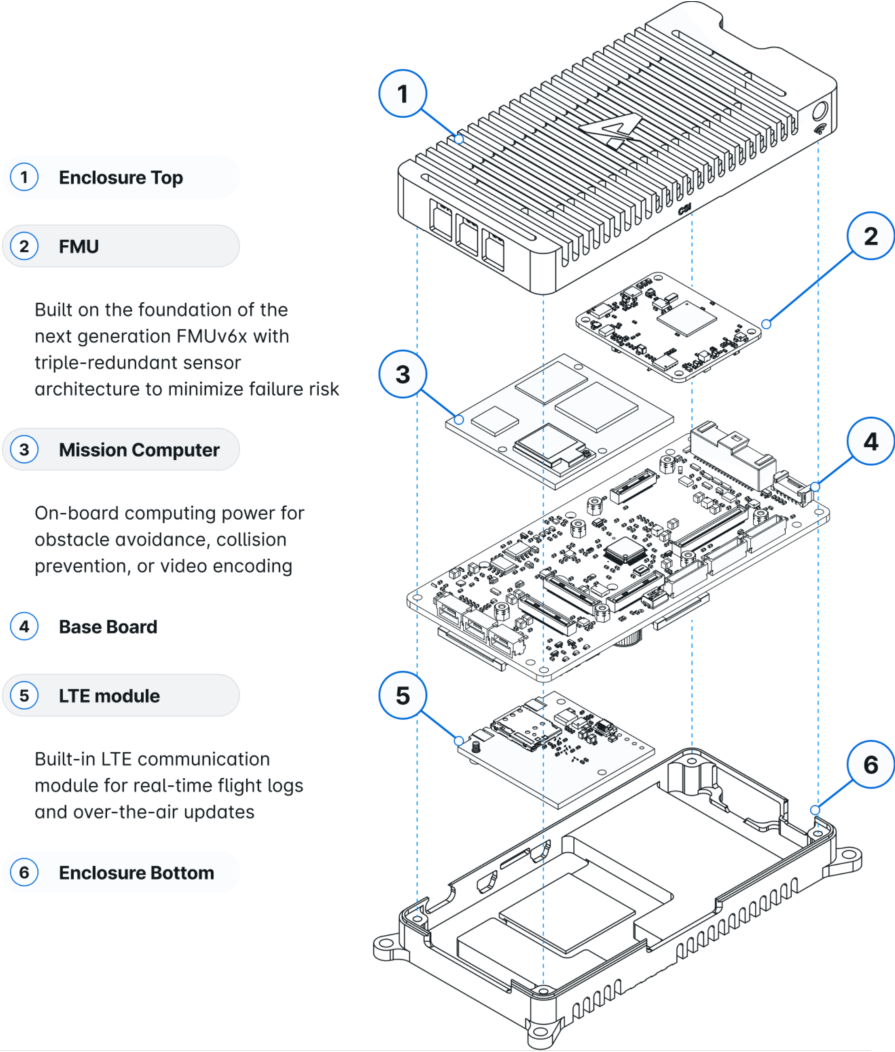
\includegraphics[width=0.8\textwidth]{./img/pdf/skynodeX-datasheet-hw.pdf} 
% %  \includesvg[width=1.0\textwidth]{./img/virtualization.svg} 
%   %\caption[Virtualization mind map]{Virtualization mind map}%
%   \caption{Auterion Skynode X}%
%   \label{fig:skynode-x-hw}
% \end{figure}
%
The mission computer comprises a ARM Cortex-A53 Quad core \gls{cpu} running at
1.8 GHz and two embedded \glspl{gpu} -- GCNanoUltra for 3D acceleration and GC320 for
2D acceleration -- with 4 GB \gls{ram} and 16 GB (\gls{emmc}) + 128 GB (internal
\gls{sd} card) of storage~\cite{skynodeXDatasheet}. Wi-Fi and Bluetooth 5 can be used for low range
wireless communications and a 4G \gls{lte} module for long range ones. It
contains Ethernet and \gls{usb} 2.0 high-speed interfaces only, as \gls{usb} 3.0 usage is discouraged
due to \gls{gps} interference~\cite{skynodeXDatasheet}.
The mission computer runs Auterion
\gls{os} (Linux-based), which communicates with the Autopilot via a proprietary
\gls{sdk} (Auterion \gls{sdk})~\cite{skynodeX-px4}.
%
It supports multicopter, \gls{vtol} airplane and airplane vehicles with a
takeoff weight of up to 500 kilograms. The price tag is circa 1900 USD
dollars\cite{skynodePrice}.

Auterion also announced in June 2024, a compact, low-cost version -- the
Auterion Skynode S -- integrating the \gls{fmu} and mission computer in a 49 x
37 millimeters footprint~\cite{skynodeS-pressRelease}. It features the FMUv6x
flight management unit from the current Skynode X family and a powerful mission
computer with a dedicated 2.3 \gls{tops} \gls{npu} for \gls{ai} and computer
vision applications~\cite{skynodeS-pressRelease}.
%
% \begin{figure}[!hbt]
%   \centering
%   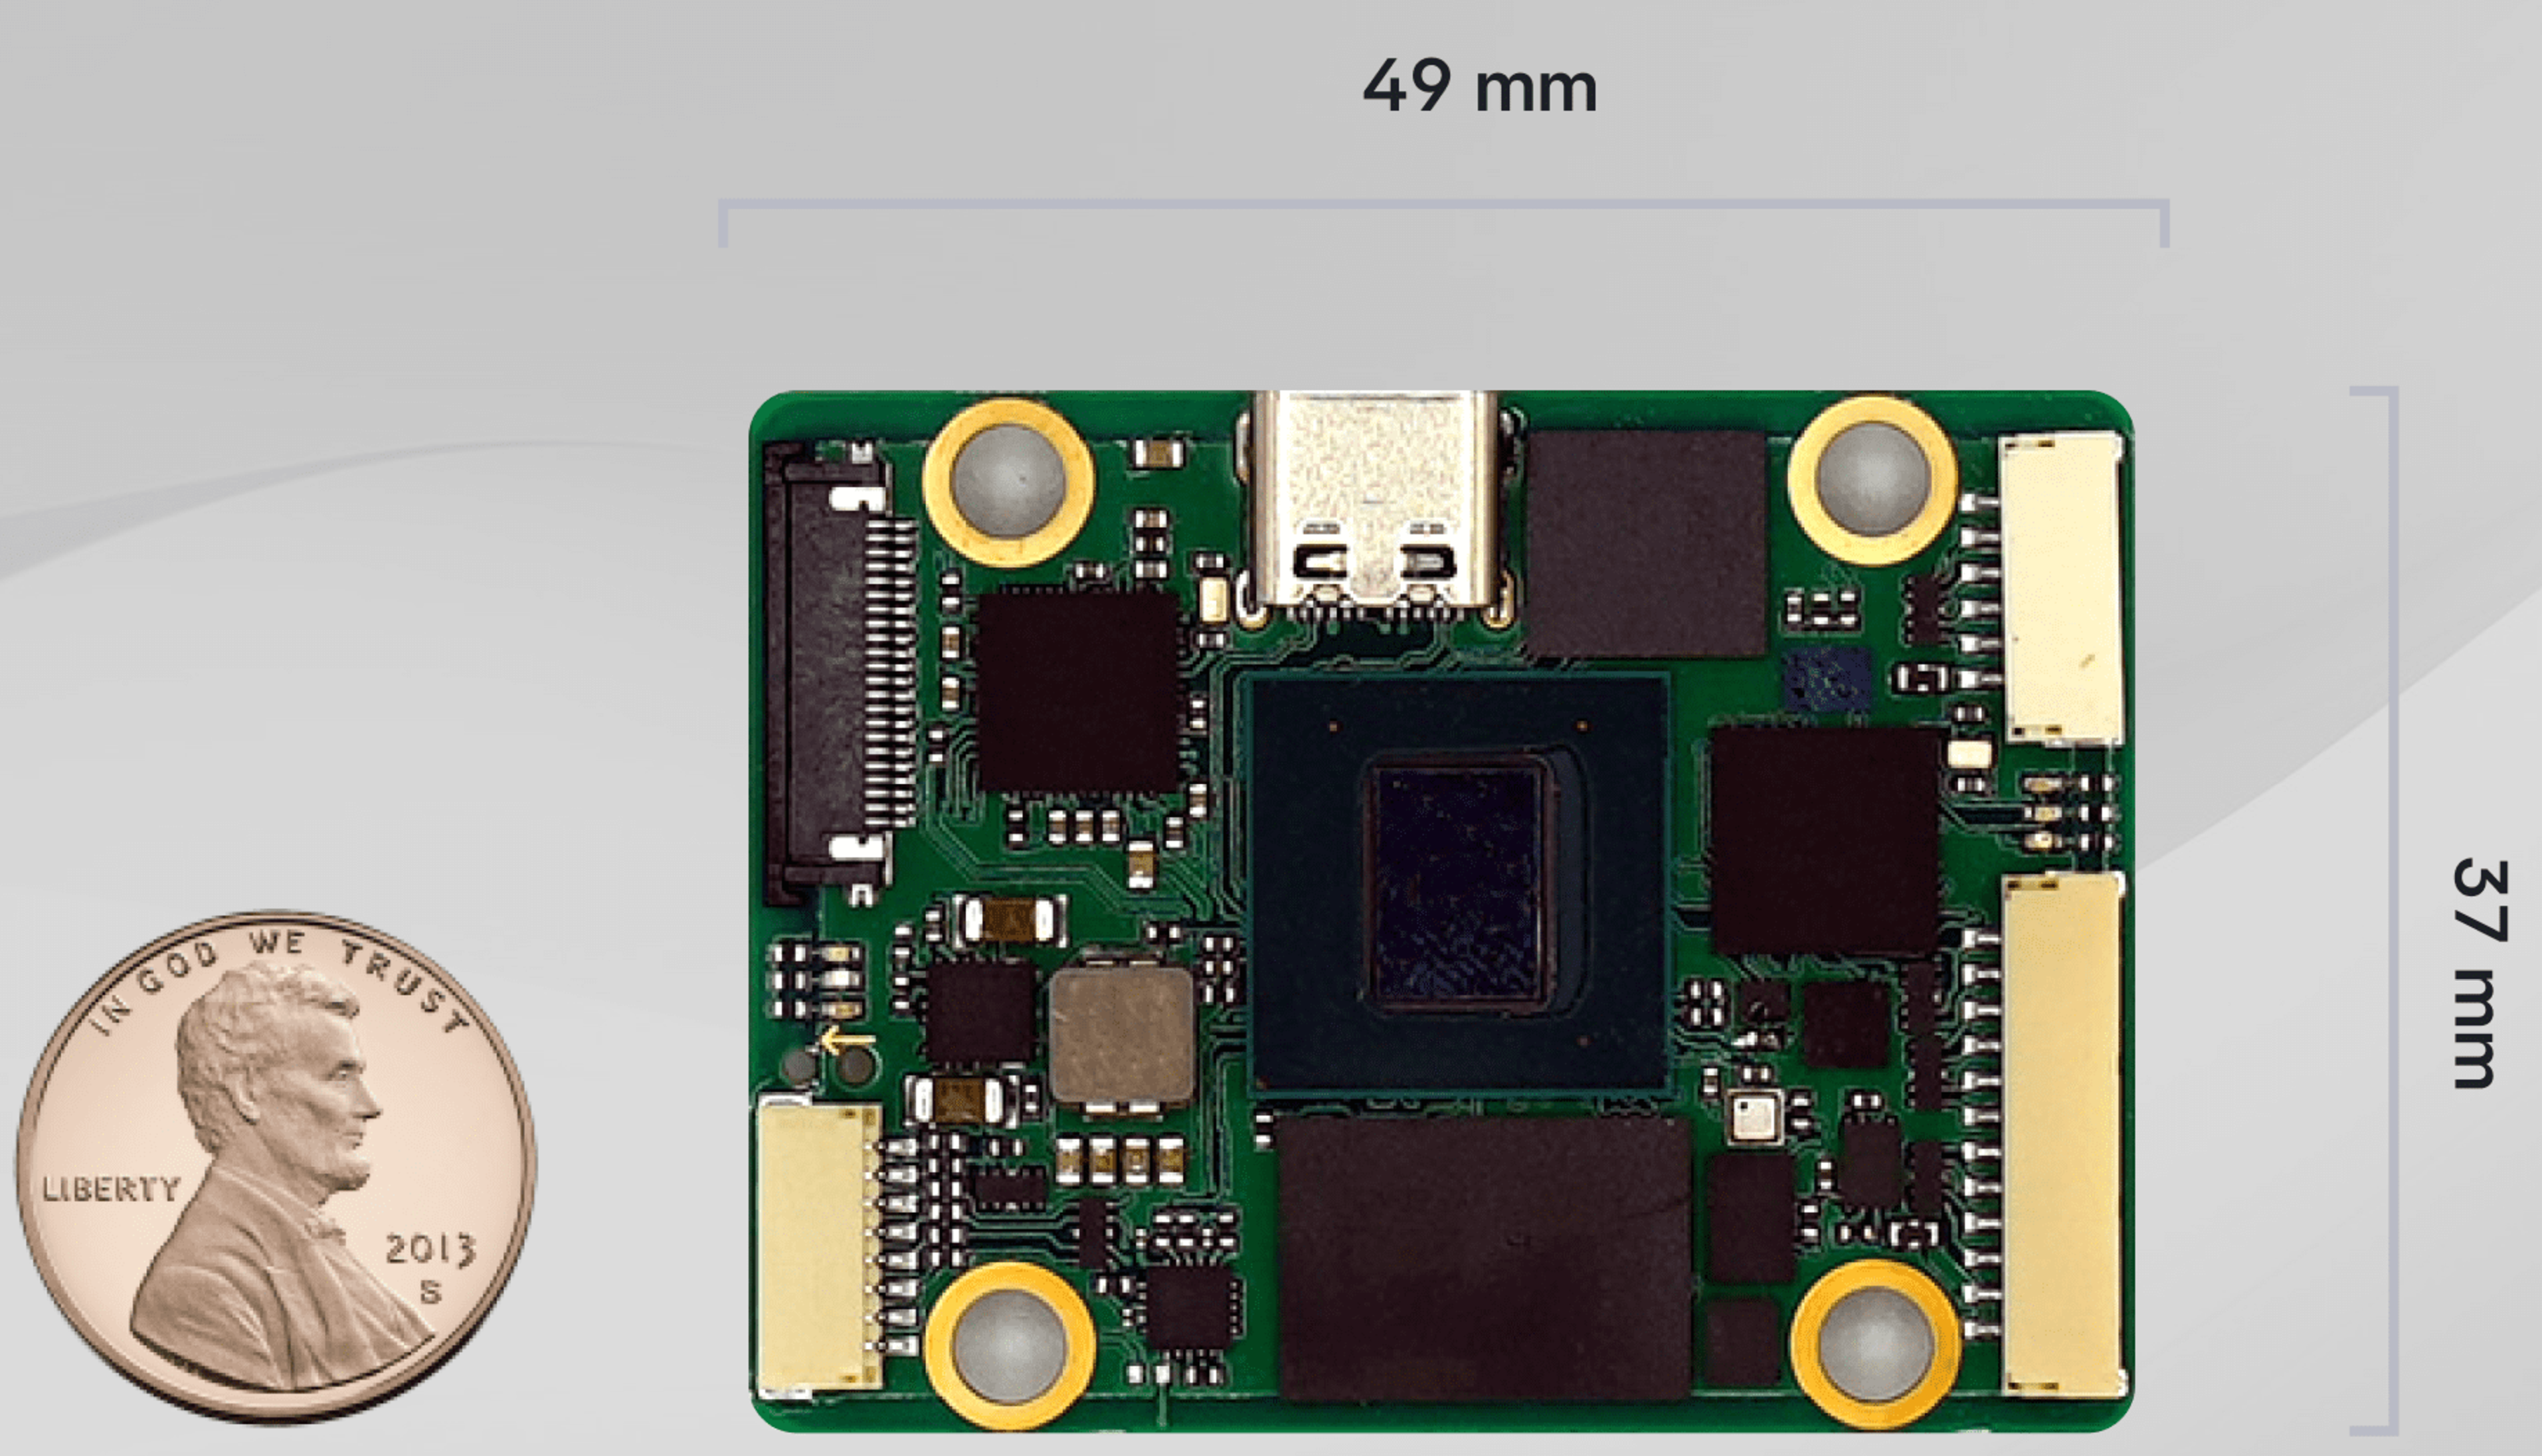
\includegraphics[width=0.8\textwidth]{./img/pdf/skynodeS-hw.pdf} 
% %  \includesvg[width=1.0\textwidth]{./img/virtualization.svg} 
%   %\caption[Virtualization mind map]{Virtualization mind map}%
%   \caption{Auterion Skynode S}%
%   \label{fig:skynode-s-hw}
% \end{figure}
%
The \gls{ai} capabilities of the Skynode S enabled the deployment of a
autonomous target tracking system, even for moving targets, which has proven its resilience against
\gls{gps} jamming or denial of service~\cite{skynodeS-noJamming}. This enabled
Ukraine to face the Russian electronic warfare, and increasing the probability
of mission's success from 20\% to 90\%~\cite{skynodeS-noJamming-2}.

% %\subsubsection{Gap analysis}%
% \label{sec:gap-analysis-hw}
% Comparison between the open-source and commercial solutions

% \begin{table}[h]
% \centering
% \small
% \caption{UAV Hardware Gap Analysis}
% \label{tab:hw-gap-analysis}
% \begin{tabularx}{\textwidth}{|l|X|X|X|}
% \hline
% \textbf{Dimension} & \textbf{Open-Source Solutions} & \textbf{Commercial Solutions} & \textbf{Gap} \\
% \hline
% Transparency & Full hardware design disclosure (schematics, BOM, PCB layouts) & Proprietary designs with limited disclosure & Open-source provides full auditability; commercial lacks transparency \\
% \hline
% Processor Architecture & ARM-based MCUs (Cortex-M7/M3 @ 216-400MHz) & Mixed: MCUs, FPGA+ARM SoCs, or integrated mission computers (Quad-core A53 + NPU) & Commercial offers higher compute diversity (FPGA/NPU) \\
% \hline
% Memory & Limited (2MB Flash/512KB RAM max) & Expanded resources (4GB RAM + 128GB storage in Skynode) & Commercial solutions offer >100× memory capacity \\
% \hline
% Sensors & Basic IMU/barometer/magnetometer & Advanced redundancy (triple IMU/GPS) and AI-capable sensors & Commercial enables fault tolerance and AI processing \\
% \hline
% Connectivity & UART/SPI/I²C/CAN & Enterprise features: LTE, VPN, Ethernet switches & Commercial provides industrial-grade networking \\
% \hline
% AI Capabilities & None & Dedicated NPUs (2.3 TOPS) for computer vision & Commercial enables edge AI for GPS-denied navigation \\
% \hline
% Power Management & Not specified & Triple-redundant power systems & Commercial prioritizes fail-safe power \\
% \hline
% Price & Low-cost (COTS components) & Premium pricing (\$1,900 for Skynode X) & 10-100× cost difference \\
% \hline
% License & Permissive (BSD) or restrictive (GPL) & Proprietary or OSS-based proprietary extensions & Commercial leverages permissive licenses for closed ecosystems \\
% \hline
% Target Market & Academic/hobbyist & Enterprise/military & Commercial focuses on mission-critical applications \\
% \hline
% \end{tabularx}
% \end{table}

\subsection{UAV Reference Software}%
\label{sec:uav-ref-sw}
In this section we discuss the reference software for \glspl{uav}.
Firstly, we present an overview over the \gls{sw} architecture. Then, we analyze
in more depth the open-source and commercial software solutions for \glspl{uav}.

\subsubsection{Overview and Architecture}%
\label{sec:overv-arch-sw}
Fig.~\ref{fig:uav-sw-arch} illustrates the high-level abstraction of the
most common structure of \gls{uav} \gls{sw}
architecture~\cite{leccadito2018survey,px4-sysArch}.
%
The main computing platforms are depicted in orange: (1) the flight controller
or \gls{fmu} (e.g., Pixhawk); (2) the \gls{gcs} (e.g., a desktop/laptop computer);
(3) and, optionally, the companion computer (e.g., a Raspberry Pi).
The companion computer provides additional features, but crucial for autonomous
flights, such as collision avoidance and prevention, odometry or payload control
(camera, \gls{lidar}, etc.). Furthermore, the companion computer can assist in
the \gls{uav}'s navigation in \gls{gps}-denied and/or communications-denied
environments, using \gls{ai}-based software components (e.g., Auterion
Skynode~\cite{skynodeS-noJamming}).
%
The physical \gls{hw} is depicted in purple (sensors, actuators, and payload),
while the layers of the \gls{sw} stack are shown in green. The arrows indicate the communication link and
associated protocols.

% UAV SW Arch
\begin{figure}[!hbt]
  \centering
  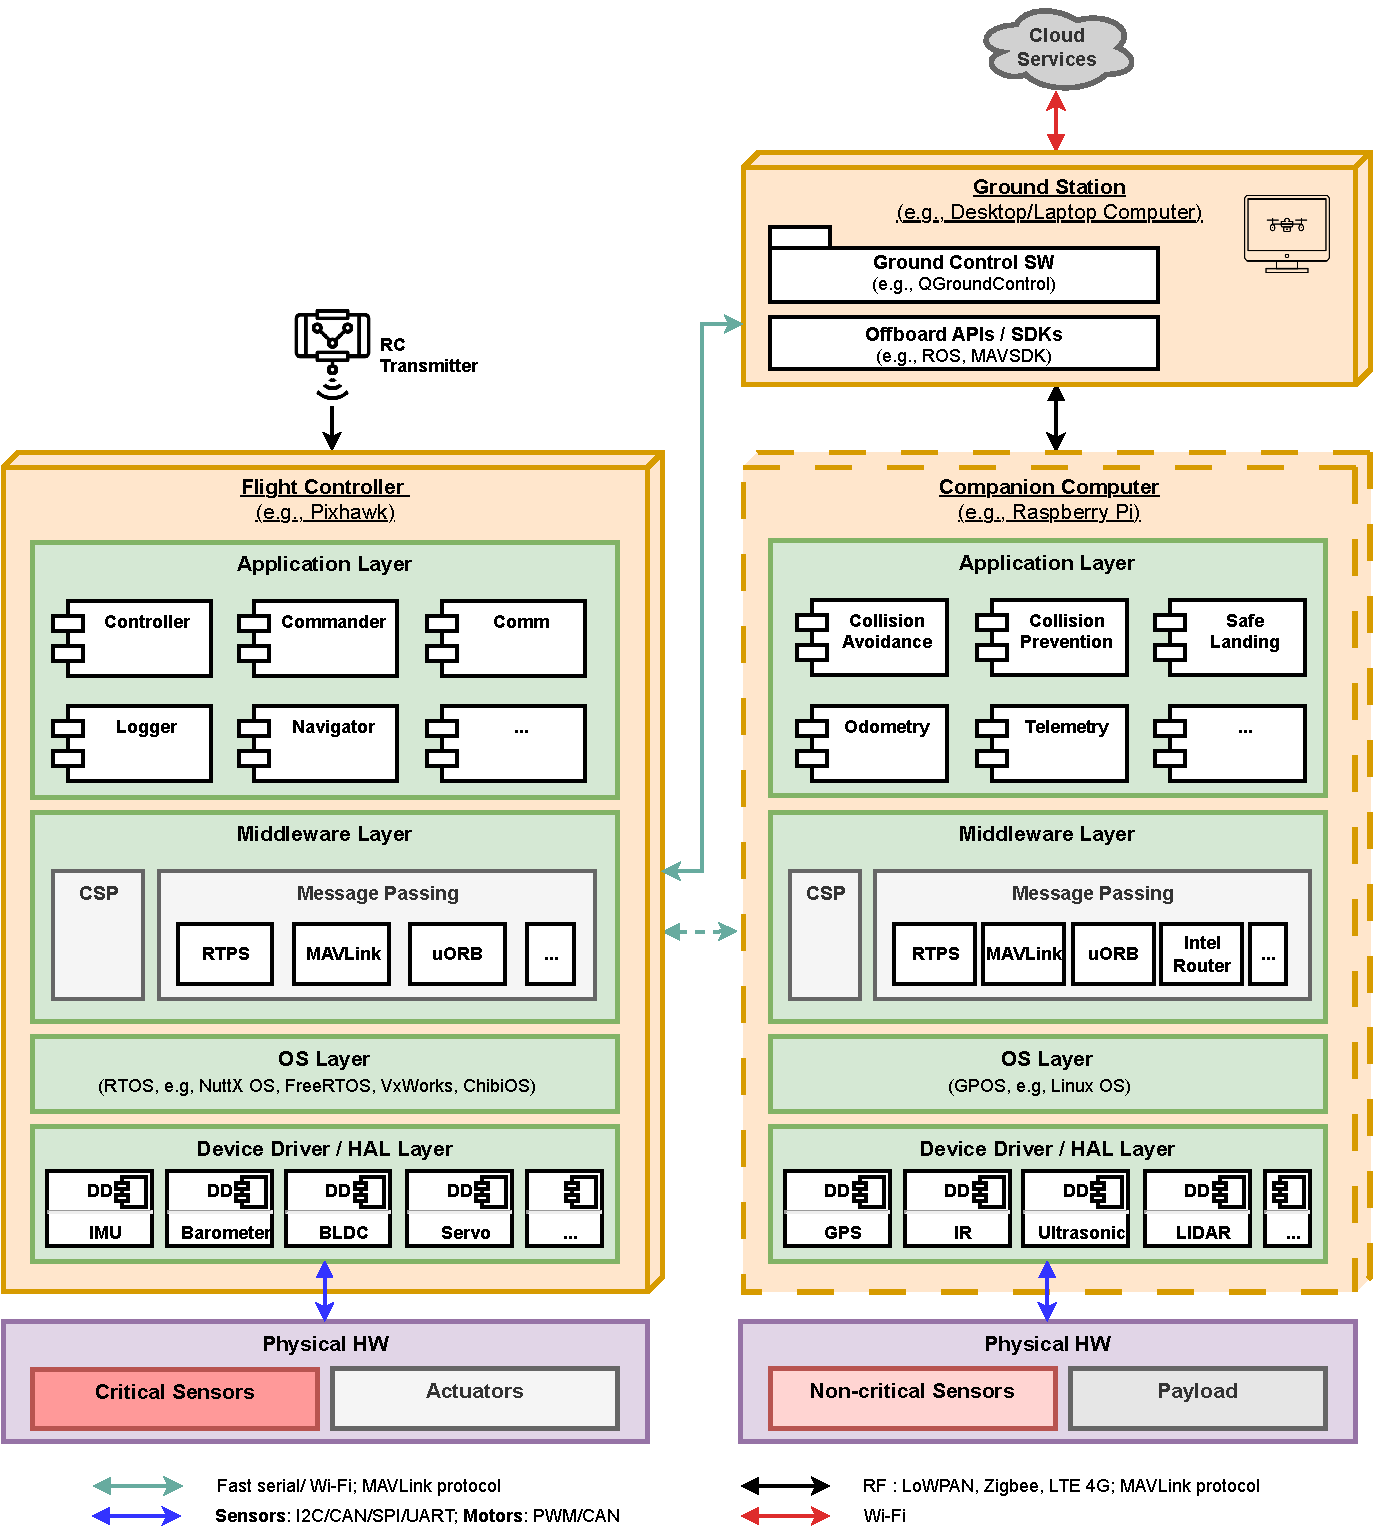
\includegraphics[width=1.0\textwidth]{./img/pdf/uav-sw-arch.pdf} 
%  \includesvg[width=1.0\textwidth]{./img/virtualization.svg} 
  %\caption[Virtualization mind map]{Virtualization mind map}%
  \caption{UAV SW architecture: most common structure}%
  \label{fig:uav-sw-arch}
\end{figure}

The flight controller and companion computer \gls{sw} stack structure is
similar, and is comprised of four layers:

\begin{enumerate}
\item \textbf{Application Layer}: this layer is where the applications/tasks
  reside, providing the high-level functionalities of the system. In the flight
  controller we have the critical tasks, namely,
  \emph{Controller}, \emph{Commander}, \emph{Navigator}, \emph{Logger},
  or \emph{Communications}, and in the companion computer the secondary tasks,
  providing mission and navigation extra features, such as, \emph{Collision
    Avoidance}, \emph{Collision Prevention}, \emph{Safe Landing},
  \emph{Odometry}, and \emph{Telemetry}.
%
\item \textbf{Middleware Layer}: the middleware is an intermediate layer,
  responsible for abstracting the interface with the \gls{os} and the
  communications through message passing --- using real-time and or asynchronous
  protocols, such as \gls{rtps}, MAVLink, or \gls{uorb} --- and for providing
  an extra layer of security enforcing \gls{csp} mechanisms. The flight
  controller communicates with the \gls{gcs} through a Wi-Fi connection and
  optionally with the Companion Computer through a fast serial/Ethernet
  connection.
%
\item \textbf{\gls{os} Layer}: the \gls{os} provides the basic services for
  system's operation and a straightforward environment for application's
  development. The flight controller hosts a \gls{rtos} to meet the stringent
  requirements and deadlines of the \gls{uav}'s control, such as,
  \lstinline{NuttX}, \lstinline{FreeRTOS}, \lstinline{VxWorks}, and \lstinline{ChibiOS}. On
  the other hand, the companion computer hosts a \gls{gpos}, as the applications
  on top have soft real-time requirements. Furthermore, it provides a much
  better bootstrapping environment for ``general'' software development than a
  \gls{rtos}, e.g., \gls{ros}-based avoidance libraries are available for Linux~\cite{px4-sysArch}.
%
\item \textbf{Device Driver Layer (\gls{hal})}: this layer abstracts the
  underlying \gls{hw}, providing a tractable interface for the \gls{os} for data
  acquisition and motors' actuation.
\end{enumerate}

The \gls{gcs} \gls{sw} (e.g., \emph{QGroundControl}) typically runs on a desktop/laptop computer or mobile
device providing real-time monitoring of the flight superimposed on a map and
\gls{uav}'s control functionalities, communicating directly with the flight
controller or indirectly via companion computer. The
\gls{sw} interface between both systems is achieved through the use of off-board
\glspl{api} or \glspl{sdk}, like \gls{ros} or MAVSDK~\cite{px4-sysArch}. 

\subsubsection{Open-source solutions}%
\label{sec:open-source-solut-sw}
\glsxtrfull{oss} solutions, like their \gls{hw} counterparts, have been
developed to provide more transparency, flexibility, and
maintainability, while trying to be cost-effective. \gls{oss} means that the
\gls{sw}'s source code is released under free/libre
terms~\cite{freeGNU}. The most prominent \gls{oss} autopilots at the moment are
\lstinline{PX4}~\cite{px4-github},
\lstinline{ArduPilot}~\cite{arduPilot-github}, and
\lstinline{Paparazzi UAS}~\cite{paparazzi-github}.
Other flight-control software, such as
\lstinline{Betaflight}~\cite{betaflight-github},
\lstinline{Cleanflight}~\cite{cleanflight-github}, and
\lstinline{Crazyflie}~\cite{crazyflie-home}, targets the \gls{fpv} racing
market and assumes expert manual piloting skills. In this context, manual
control is the priority, so autopilot features are generally unnecessary and not
supported.
%
%
% \paragraph{PX4}
%
\lstinline{PX4} is an autopilot flight stack for \glspl{uv}, with a strong focus on the
\glspl{uav}. Started in 2012 and released under
a permissive \gls{bsd}-2 license~\cite{px4-github}, it is widely used in
industrial and commercial domains
\lstinline{PX4}~\cite{skynodeX-px4,spRacing-px4}. Like ArduPilot, it supports a
broad range of \gls{uav} airframes and other \glspl{uv}.
%
PX4 is loaded onto
the flight controller \gls{hw} using the \emph{QGroundControl}
application and runs atop of the NuttX OS, although ROS support is also
available~\cite{jargalsaikhan2022architectural}. \emph{QGroundControl} is also
used to configure PX4 and interface the flight controller, and an \gls{rc} unit
can be used to manually control the drone.
%
PX4 uses the MAVLink protocol to communicate with the flight controller and the
\gls{uorb} message \gls{api} for data transfer between its internal
modules~\cite{px4-sysArch,jargalsaikhan2022architectural}. It requires an
\gls{imu}, magnetometer and barometer for manual modes, but for autonomous
missions a \gls{gps} must be used. Flight logs are generated upon takeoff and
can be analyzed to assess the flight behavior using \emph{Flight Review}, or
\emph{Px4Tools}~\cite{glossner2021overview}. 

%\paragraph{ArduPilot}
%
\lstinline{ArduPilot} is another autopilot flight stack for \glspl{uv}, also with a strong focus
on \glspl{uav}. Started in 2009, it was released under the more restrictable
\gls{gpl}v3 license~\cite{arduPilotHistory}. It supports the \emph{Linux} and
\emph{ChibiOS} operating
systems~\cite{arduPilot-github,jargalsaikhan2022architectural} and runs on a large number of
\gls{osh} platforms such as \emph{Pixhawk}.
%
ArduPilot features, like PX4~\cite{px4-features}, include:
multiple flight modes (manual, semi- and full-autonomous) with multiple
stabilization options; programmable missions with 3D waypoints and optional
geofencing; support for multiple sensors and buses; fail-safe actions and
support for navigation in \gls{gps} denied environments~\cite{arduPilot-home}.
%
ArduPilot supports the MAVLink protocol for communication with
\glspl{gcs} and companion computers~\cite{arduPilot-home}. Mission commands are
stored in \gls{eeprom} and executed one-by-one when the vehicle is switched into
\emph{Auto} mode~\cite{ardupilot-mavlink}.

% \paragraph{Paparazzi UAS}
%
\lstinline{Paparazzi UAS} is the oldest autopilot flight stack for drones
currently active. Started in 2003, it was released under the \gls{gpl}v2
license, supporting different \gls{uav}'s airframes~\cite{paparazzi-home}.
It runs atop of the \emph{ChibiOS} operating
system~\cite{paparazzi-sysOverv} and uses its own \emph{PPRZLINK} protocol for communication
with \glspl{gcs} and companion computers~\cite{paparazzi-sysOverv}, transferring
data between the modules via the proprietary middleware \emph{AirBorne Ivy} \gls{abi}~\cite{jargalsaikhan2022architectural}.

% \paragraph{}
Jargalsaikhan et al.~\cite{jargalsaikhan2022architectural} surveyed
flight-control software portability at the module level. They examined the
overall structure, messaging mechanisms and supported \gls{os} in academic and \gls{oss} solutions and compared them against portability requirements:
simplicity, modularity, centralized messaging, standard interfaces, \gls{hal}
implementation, and documentation. The authors concluded the following: (1) only
\emph{ArduPilot} and \emph{PX4} implement a \gls{hal}; (2) \emph{ArduPilot}
lacks a message-centralization mechanism; (3) despite being open source, all
surveyed systems use proprietary messaging interfaces, which hinders
portability; (4) and documentation, while generally available, is sometimes hard
to understand or partially outdated. Fig.~\ref{fig:uav-sw-arch-oss-compar} shows the \gls{sw}
stack layers and modules for the aforementioned \gls{oss} solutions and for
\emph{mpFCS}, the portable \gls{fcs} developed by Jargalsaikhan et
al.~\cite{jargalsaikhan2022architectural}.


% UAV SW Arch OSS Comparison
\begin{figure}[!hbt]
  \centering
  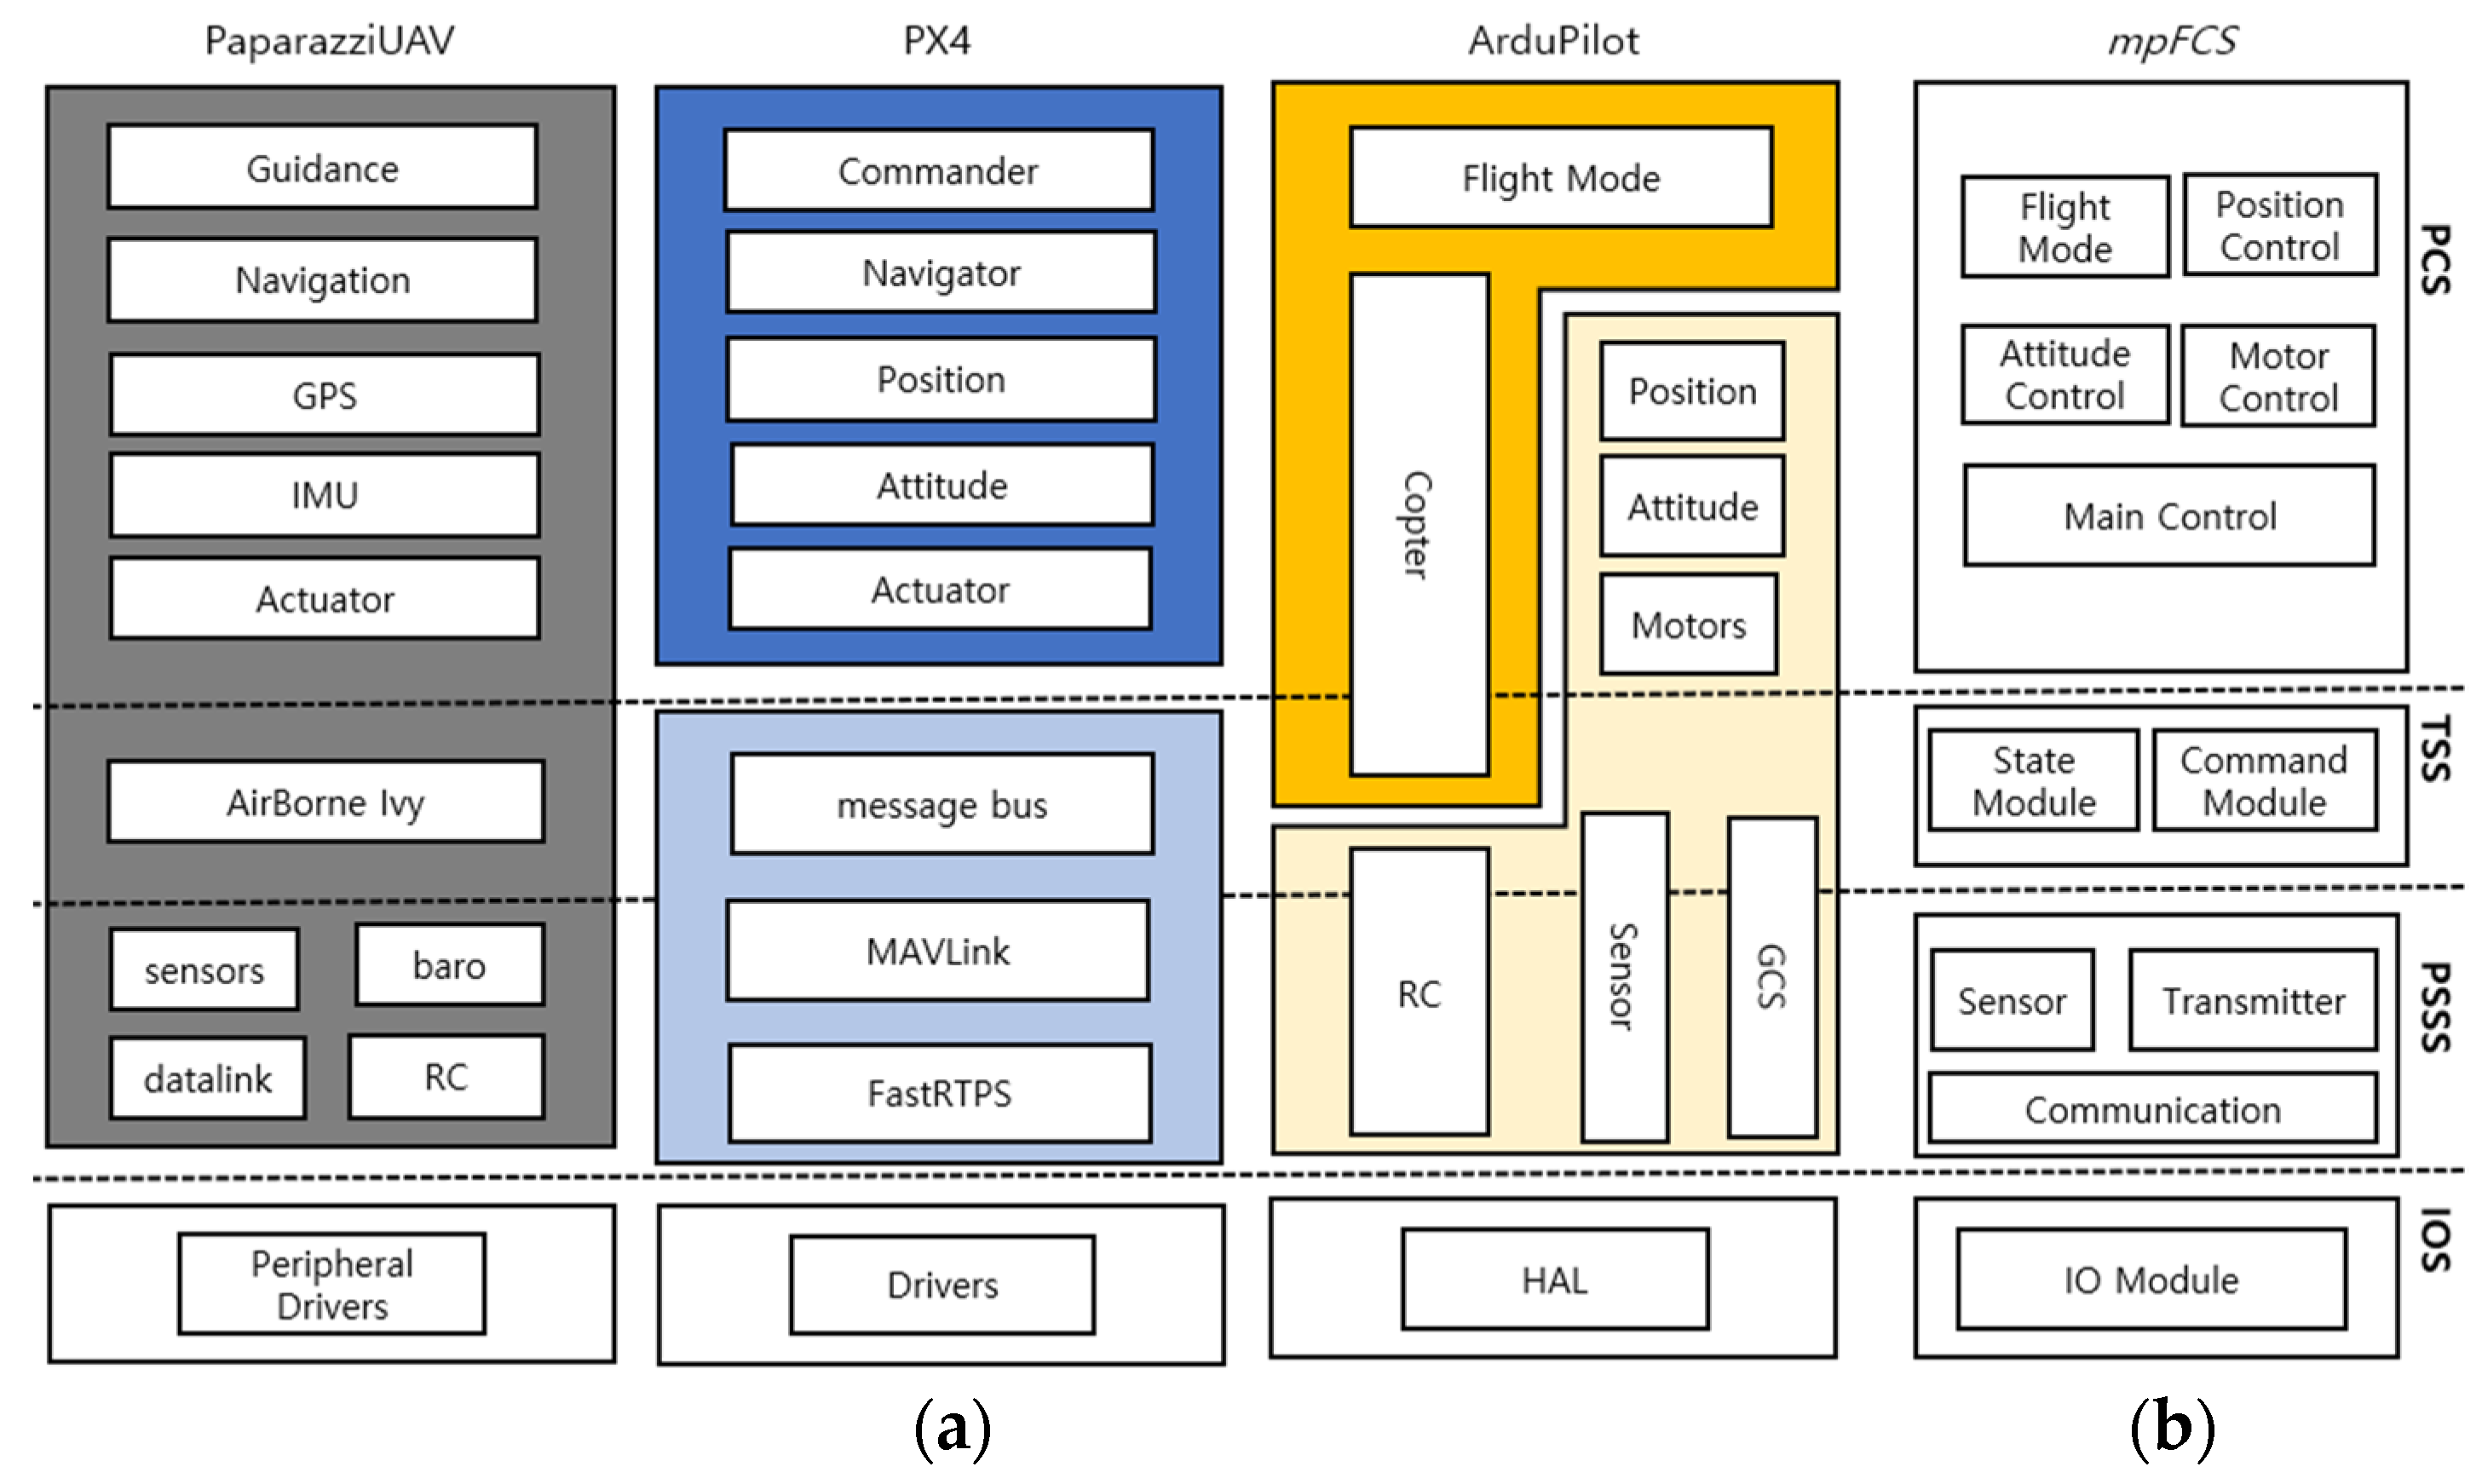
\includegraphics[width=0.8\textwidth]{./img/png/uav-sw-arch-oss.png} 
%  \includesvg[width=1.0\textwidth]{./img/virtualization.svg} 
  %\caption[Virtualization mind map]{Virtualization mind map}%
  \caption[Analysis of the OSS modules and the mpFCS]{Analysis of the OSS
    modules and the mpFCS:~(a) OSS (Paparazzi UAS, PX4, ArduPilot); (b) mpFCS~\cite{jargalsaikhan2022architectural}\footnotemark}%
  \label{fig:uav-sw-arch-oss-compar}
\end{figure}
 % TODO: get license
\fnlicReq{MDPI}{5457890117132}%

\subsubsection{Commercial solutions}%
\label{sec:commercial-solutions-sw}
Typically, the commercial proprietary solutions do not disclose information
about the product. They provide extensibility through the use of
\glspl{sdk}, like the Dji~\cite{djiSDK} or the Parrot drones\cite{parrot-sdk}, enabling the end-user to use
extra features, but requires specialized knowledge.
%
On the other hand, some commercial solutions can explore
more permissible \gls{oss} licenses, like the \gls{bsd} license provided by PX4,
to add extra functionalities and bundle it as a closed, commercial,
product. This is exactly the case for the Auterion PX4 (PX4) autopilot, a
enterprise-hardened autopilot that runs on the Auterion \glspl{fmu}.
Fig.~\ref{fig:uav-sw-arch-auterion} illustrates the Auterion software stack.

% UAV SW Arch
\begin{figure}[!hbt]
  \centering
  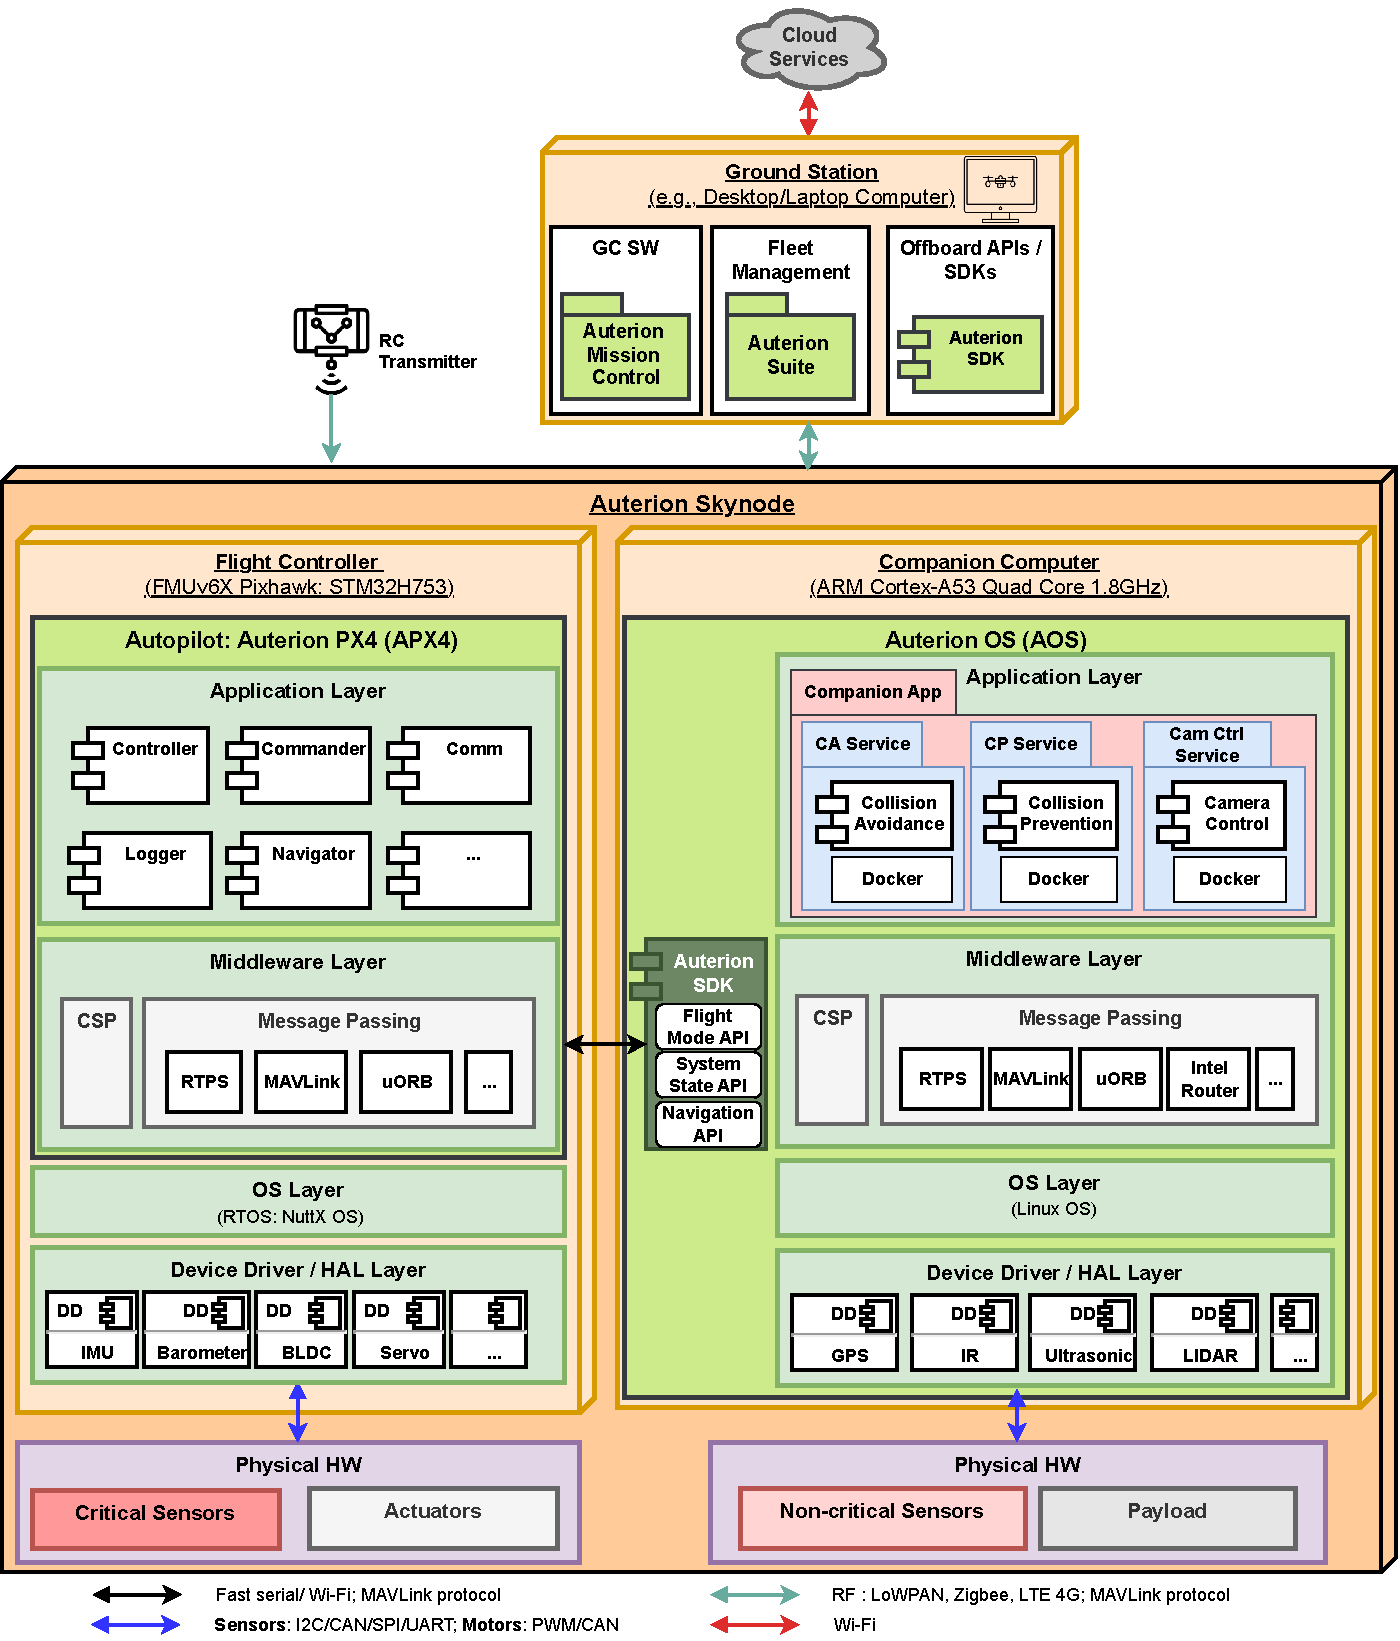
\includegraphics[width=1.0\textwidth]{./img/pdf/uav-main-sw-arch-auterion.pdf} 
%  \includesvg[width=1.0\textwidth]{./img/virtualization.svg} 
  %\caption[Virtualization mind map]{Virtualization mind map}%
  \caption{UAV SW architecture: Auterion software stack}%
  \label{fig:uav-sw-arch-auterion}
\end{figure}

The \lstinline{Auterion Skynode} combines the an FMUv6X-based Pixhawk
\gls{fmu} and the companion/mission computer into a single board~\cite{auterion-sw}. The flight
controller runs the autopilot stack (APX4) on top of the NuttX \gls{rtos}
licensed under the Apache 2.0 license which allows for proprietary reuse. The
mission computer runs the Auterion \gls{os} (AOS), a customized embedded Linux
\gls{os}, to support additional features, like collision avoidance and
prevention, odometry, or camera control~\cite{auterion-sw}. These additional features or services,
are containerized in a Docker image to increase isolation and enable easy and
fast system update, minimizing the dependencies. However, to optimize storage
requirements, developers are instructed to: (1) package these services into a
single application (e.g., \lstinline{Companion App}), ensuring the user only needs to handle a single
\lstinline{.auterionos} file; (2) write a common base \lstinline{Dockerfile} for
a shared environment for the deployed services~\cite{auterion-sw-services}. Thus, AOS software development
follows the microservices architecture based on the Docker technology.
The AOS' applications can query the autopilot or issue commands to it using the
provided \glspl{api} in the \lstinline{Auterion SDK}.
%
The \lstinline{Auterion Skynode} can be controlled using a \gls{rc} transmitter
or software running on the \gls{gcs}. The \lstinline{Auterion Mission Control}~\cite{auterion-missionControl}
is a ground control software specialized for Auterion vehicles, very similar to
\lstinline{QGroundControl}, enabling the UAV's remote control.
The \lstinline{Auterion Suite}~\cite{auterion-suite} is a fleet management \gls{sw}, providing
real-time information about the UAV, predictive maintenance actions, flight
analysis, and \gls{ota} updates.

If, however, we expand the search to include any proprietary
software component, such as the \lstinline{VxWorks} \gls{rtos} then the results'
list becomes significantly larger, namely, the Northrot Grumman X-47B
\gls{uav}~\cite{vxWorks-uav-northrop}, the Airbus
Helionix~\cite{vxWorks-uav-aribus-helionic}, and the Airbus
Atlante~\cite{vxWorks-uav-aribus-atlante}.
%

% \subsubsection{Gap analysis}%
% \label{sec:gap-analysis-sw}
% Comparison between the open-source and commercial solutions

% \begin{table}[h]
% \centering
% \small
% \caption{UAV Software Gap Analysis}
% \label{tab:sw-gap-analysis}
% \begin{tabularx}{\textwidth}{|l|X|X|X|}
% \hline
% \textbf{Dimension} & \textbf{Open-Source Solutions} & \textbf{Commercial Solutions} & \textbf{Gap} \\
% \hline
% License & GPL/BSD licenses with source access & Proprietary SDKs or OSS-based closed products & Commercial restricts modification rights \\
% \hline
% Middleware & Custom protocols (uORB, PPRZLINK) & Standardized microservices with Docker containers & Commercial offers modern containerization \\
% % \hline
% % Portability & Limited HAL implementation & Enterprise-hardened portability & Commercial provides production-grade abstraction \\
% \hline
% API Extensibility & ROS/MAVSDK support & Proprietary SDKs with cloud integration & Commercial enables tighter ecosystem control \\
% \hline
% Real-Time Performance & RTOS-based (NuttX, ChibiOS) & Military-grade RTOS (VxWorks) & Commercial offers certified real-time guarantees \\
% \hline
% Update Mechanism & via USB or radio in offline mode & via USB, radio or Wi-Fi; updates with fleet management & Commercial enables remote maintenance \\
% \hline
% Security Features & Basic CSP mechanisms & Container isolation + hardware-enforced security & Commercial provides defense-grade protection \\
% \hline
% AI/ML Integration & Limited (ROS-based libraries) & Native AI stack for target tracking & Commercial enables advanced autonomous behaviors \\
% \hline
% Ecosystem Tools & QGroundControl + Flight Review & Integrated mission control + cloud suites & Commercial offers end-to-end mission lifecycle support \\
% \hline
% Documentation & Partially outdated & Professional technical support & Commercial ensures reliability for critical ops \\
% \hline
% \end{tabularx}
% \end{table}

\section{Related work}%
\label{sec:related-work}
\glspl{uav}'s market is booming, but the security and safety is often overlooked
in the design~\cite{ferrao2020stuart}. Several vulnerabilities have been
identified~\cite{kishnaCyberVulnerUAVReview2017,nassi2021sok,mohsan2022towards},
with a extensive attack surface area --- \gls{fcs}, \gls{gcs}, chassis, \gls{fpv}
channel, and the cloud services.

The commercial \gls{sw} solutions do not provide the security mechanisms
required, and, furthermore lack transparency. 
%
Buquerin~\cite{buquerin2018security} conducted a security evaluation on the
VxWorks 7 \gls{rtos} --- a commercial professional-level \gls{rtos} --- for
avionic systems. The author reported that basic attacks such as
buffer overflows or string vulnerabilities led to a noticeable performance
decrease in the system. Moreover, no security mechanism protects the system
from malware or command injection vulnerabilities. This poses a major threat on
the system if no supervising technology, like virtualization, is used. On the other hand, good security practices are used in
areas such as cryptography and privilege management.
To mitigate this issue, Auterion employs in the mission computer a microservices architecture based on
application containerization using the Docker
technology~\cite{auterion-sw-services}. However, as all applications share the
same host \gls{os} kernel, a misconfigured or ill-behaving application can
compromise the mission computer, and inject erroneous commands into the
autopilot, compromising the whole system. Furthermore, the autopilot runs
unsupervised on the flight controller, i.e., it typically has full access to all
of the hardware resources, increasing the attack surface area. Executing the
autopilot in supervised mode, namely with static partioning of resources, can
mitigate this issue by enforcing the User to carefully select the appropriate
hardware for each mission, but also by trapping, and thus preventing, any ill-intentioned access to unavailable hardware resources.

With the open-source solutions, comes transparency, but, nonetheless, it is
insufficient to meet the mixed-criticality and security requirements.
Zhang et al.~\cite{zhang2021best} compared the two main \glspl{rtos} for drone's applications in the
open-source domain, Nuttx and ChibiOS, with the latter emerging as the best. Not
only ChibiOS outperforms NuttX in most temporal tests, but also, and even more
importantly, succeeds in the priority inversion avoidance test with mutexes
rather than binary semaphores. The context switch overhead is greater for
the NuttX, augmenting the probability of missing deadlines. Furthermore, NuttX
does not provide priority inheritance using mutexes, which may lead to faulty
designs, and has a larger codebase. Since \glspl{uav} have stringent real-time
constraints, ChibiOS appears to the be the best \gls{rtos} for \glspl{fcs}, and
therefore the migration of ArduPilot's from NuttX to ChibiOS is probably a smart
decision.

This leads to some research being conducted on changing the paradigm entirely.
Alladi et al.~\cite{alladi2022UAVBlockain} propose a completely different
approach --- the use of a decentralized architecture to increase security in
\glspl{uav} application through the application of blockchain --- especially in
cooperative environments. Blockchain features such as smart contracts and
consensus mechanisms and the inherent cryptographic foundations, enabling
automation and providing security, according to the authors. Overall, the
blockchain technology helps in overcoming many problems such as coordination,
security, collision avoidance, privacy, decision making, and signal
jamming. Although it presents great potential, the real-life implementation
seems a little distant.

On the other hand, virtualization is a well-proven and mature technology,
emerging as a viable solution to handle the \gls{uav}'s
mixed-criticality requirements and security, through spatial, temporal, and
fault isolation. Nonetheless, the number of works in these field is still scarce.
Faultrel et al~\cite{fautrel2019hypervisor} proposed an hypervisor based
approach for mixed critical real-time \gls{uav} applications to meet its
stringent timing and criticality requirements and allow \gls{fcs}
certification. The authors used an iterative approach for the construction of
scheduling tables at the hypervisor level. This approach was then applied to the
use case of an industrial project of inspection drone systems comprising three
\glspl{vm} of different criticality levels: (1) high -- autopilot, running on baremetal; (2) medium --
communication application between the \gls{gcs} and the \gls{uav}, running on OpenWRT; (3) low --
video application that stores, analyzes, and compresses images, running on a
Linux Debian \gls{os}. The authors used the PikeOS level 1 hypervisor as it can
be certified DO 178B/C for flying systems. However, PikeOS is closed source,
hindering the widespread adoption to small and inexpensive \gls{uav} systems.

It is important to note that virtualization is also broadly used in the literature to encompass the usage of
\gls{uav} in larger, adaptable networks, where each \gls{uav} can provide
different services depending on a dynamic configuration. This is also referred
to as softwarization of \gls{uav} networks~\cite{oubbati2020softwarization}. For
example, Nogales et.~al~\cite{nogales2018adaptable} proposed the deployment of
small \glspl{uav} capable of executing virtual functions and services for rapid
adaptation to different missions with heterogeneous objectives. The authors
implemented an \gls{ip} telephony service as a set of virtualized network
functions, tested with real voice-over-IP terminals.

On academia, \emph{VxWorks} was also used as \gls{rtos} for \gls{uav}
applications. Chong and Li~\cite{vxworksFCS} designed a \gls{fcs} for small
\glspl{uav} using \emph{VxWorks} as an \gls{rtos} to support tasks partitioning
meeting the real-time requirements. Fig.~\ref{fig:vxworks-sw-arch} illustrates
the software framework designed considering three main layers: functional layer
(application + middleware), \gls{os} layer, and device driver layer. The authors
claimed remarkable improvements in the reliability and real-time capability of
the \gls{fcs} using \lstinline{VxWorks}, due to its multitasking capabilities, but did not provide direct comparison with
other \glspl{rtos}.

\begin{figure}[!hbt]
  \centering
  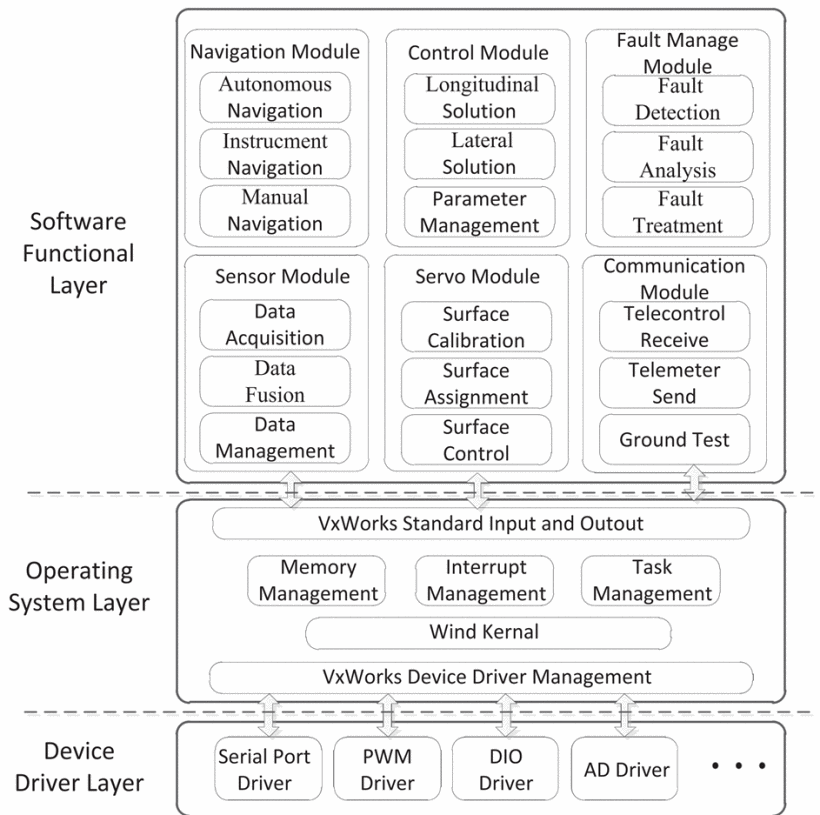
\includegraphics[width=0.8\textwidth]{./img/png/vxworks-sw-arch.png} 
  \caption[SW framework for an UAV application based on the VxWorks
    RTOS~]{SW framework for an UAV application based on the VxWorks
    RTOS~\cite{vxworksFCS}\footnotemark}%
  \label{fig:vxworks-sw-arch}
\end{figure}
%
\fnlicReq{IEEE}{5457890117132}%


% \section{Summary}%
% \label{sec:summary-state}
% \gls{uav} are being extensively deployed in a myriad of applications, such as:
% search and rescue missions, agriculture and farming, military missions,
% delivering goods and medical supplies, video capturing and filming, providing
% telecommunications in remote areas, among others. Nonetheless, vehicle's
% security and safety is often overlooked, with several documented vulnerabilities
% and an extensive attack surface area.

% The \gls{uav} architecture is typically heterogeneous by nature and with
% different criticality levels, i.e., a \glsxtrfull{mcs}, comprising a
% critical and a non-critical system. The critical system runs the autopilot
% software stack in the flight controller to control the \gls{uav}, sampling the critical sensors (\gls{imu}, gyroscope,
% compass, and barometer) and computing the required actuator values to maintain
% the navigation heading according to the specified parameters.
% The non-critical system provides additional features such as collision detection
% and avoidance or payload control. It uses a so called companion or mission
% computer for this purpose. Although optional, the companion computer is crucial
% for autonomous flights, and can be enhanced to provide \gls{ai}-assisted
% navigation in \gls{gps}-denied or communications-denied environments. A \gls{rc}
% transmitter can be used to manually operate the \gls{uav}, while the companion
% computer can command the flight controller to follow several waypoints in
% mission mode, typically using a fast serial link. The ground station runs the
% \glsxtrfull{gcs} to assist in the mission planning, but also for configuring the
% \gls{uav} and to obtain real-time flight data via telemetry radio or \gls{lte}
% link. Typically, the \gls{uav} is battery-powered, but fuel or hybrid systems
% are also common. The most notable open-source flight controllers are the
% Pixhawk (microcontroller-based) platforms, while the commercial alternatives
% range from the microcontroller-, \gls{fpga}-, or companion-based
% platforms. Perhaps, the most notable of the commercial solutions is the Auterion
% Skynode X based on the Pixhawk \gls{fmu}v6 architecture (\gls{bsd} license). It
% combines a flight controller, a mission computer and \gls{lte} connectivity in a
% compact form factor.

% Regarding the software stack, the flight controller and companion computer are
% structured similarly in four layers: application, middleware, \gls{os}, and
% \gls{hal}. The application layer provides the high-level functionality of the
% system, the middleware abstracts the interface with the \gls{os} and the
% communications through message passing, the \gls{os} provides the basic services
% for system's operation, and the \gls{hal} abstracts the underlying \gls{hw}. The
% flight controller runs the autopilot (application + middleware) (e.g., PX4 or
% Ardupilot) on top of a \gls{rtos} (e.g., NuttX, ChibiOS, VXWorks). The mission
% computer runs a \gls{gpos}, typically Linux-based. On the commercial side,
% Auterion runs an enterprise-hardened version of PX4 (APX4) on the \gls{fmu}, and
% a customized version of an embedded Linux \gls{os} (AOS). It provides an
% \gls{sdk} with the relevant \glspl{api} to enable the AOS to query and command
% the APX4. It provides a microservices architecture based on the Docker
% technology to deploy applications on top of AOS.

% The commercial \gls{sw} solutions lack security mechanisms, rendering it
% susceptible to basic attacks such as buffer overflows or strings
% vulnerabilities, or more advanced ones such as malware or command injection.
% To mitigate this issue, Auterion employs application containerization in the
% mission computer. However, as all applications share the
% same host \gls{os} kernel, a misconfigured or ill-behaving application can
% compromise the mission computer, and inject erroneous commands into the
% autopilot, compromising the whole system. Furthermore, the autopilot runs
% unsupervised on the flight controller, i.e., it typically has full access to all
% of the hardware resources, increasing the attack surface area. Executing the
% autopilot in supervised mode, namely with static partioning of resources, can
% mitigate this issue by enforcing the User to carefully select the appropriate
% hardware for each mission, but also by trapping, and thus preventing, any ill-intentioned access to unavailable hardware resources.

% Due to the wide and varied attack surface, some research focuses on changing the
% paradigm, e.g., using a blockchain decentralized architecture to mitigate many
% \gls{uav} problems such as coordination, security, collision avoidance, privacy,
% decision making, and signal jamming. 
% Although it presents great potential, the real-life implementation
% seems a little distant.

% On the other hand, virtualization is a well-proven and mature technology,
% emerging as a viable solution to handle the \gls{uav}'s
% mixed-criticality requirements and security, through spatial, temporal, and
% fault isolation. Nonetheless, the number of works in these field is still scarce
% and are based on closed source hypervisors, such as PikeOS.

% Thus, the research demonstrates the \gls{uav} software stack can benefit from
% the usage of virtualization to handle mixed-criticality requirements in a secure
% way. This is especially true for the open-source software stack. Virtualization
% provides isolation and can assist in the consolidation of the computing
% platforms, minimizing the \gls{swap-c} metrics.

%%% Local Variables:
%%% mode: latex
%%% TeX-master: "../template"
%%% reftex-default-bibliography: ("../Bibliography/mieeic.bib")
%%% ispell-local-dictionary: "american"
%%% End:
